\title[Swaq]{\color{black} \LARGE SWAQ}
\subtitle[ちょっと強いQAS]{特定の問題にちょっと強くなった量子アニーリングシミュレーター}
\author[岡田颯斗]{岡田颯斗}
\institute[大阪府立四條畷高等学校]{大阪府立四條畷高等学校}
\date{}
\begin{frame}{}
\titlepage
\end{frame}
\large

\begin{frame}
  \frametitle{目次}
  \tableofcontents
\end{frame}

%add here

\section{自己紹介}
\begin{frame}
  \frametitle{どうもこんにちは}
  \begin{columns}
    \begin{column}{0.5\linewidth}
      \begin{itemize}
        \item 名前:岡田颯斗(高校3年生)
        \item 好きなモノ
        \begin{itemize}
            \item 競技数学
            \item ナン
        \end{itemize}
        \item 興味があるコト
        \begin{itemize}
          \item 量子コンピューター
        \end{itemize}
    \end{itemize}
    \end{column}
    \begin{column}{0.5\linewidth}
      \begin{figure}
        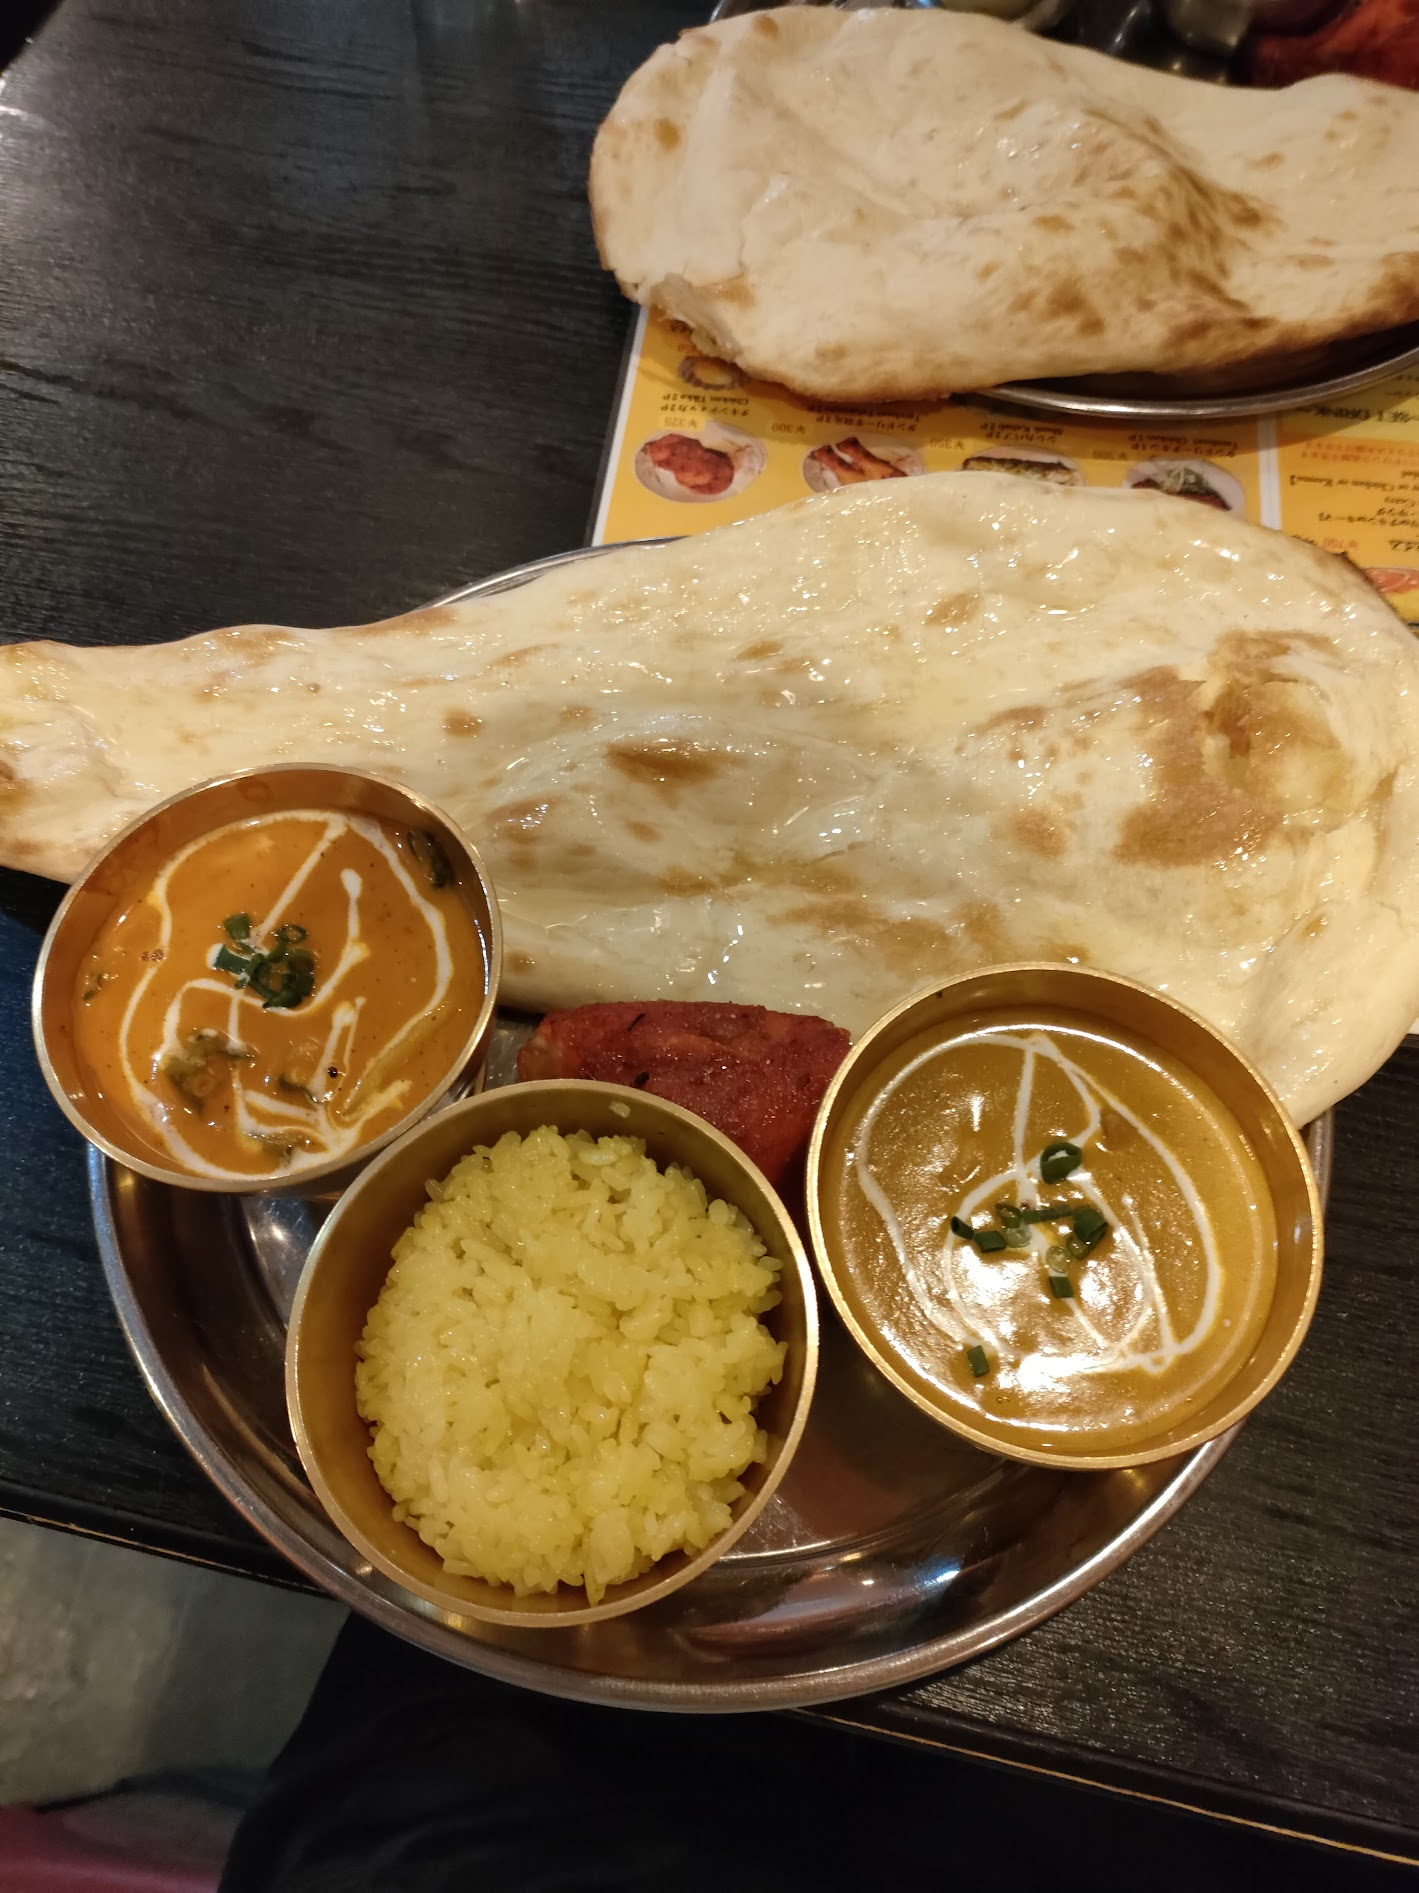
\includegraphics[width=0.7\linewidth]{data/nan}
      \end{figure}
    \end{column}
  \end{columns}
\end{frame}

\section{前提}
\begin{frame}
  \frametitle{量子アニーリングは組合せ最適化問題を解く手段の一つ\cite{Kadowaki_1998}\cite{大関真之2018量子アニーリングによる組合せ最適化}}
  よく扱われる問題の例\cite{lucas2014ising}:\\
  \vspace{10mm}
  \begin{columns}
    \begin{column}{0.45\textwidth}
      \textbf{n-彩色問題}
      \begin{itemize}
          \item 隣り合う場所は異なる色で塗分ける
      \end{itemize}
    \end{column}

    \begin{column}{0.45\textwidth}
      \textbf{巡回セールスマン問題}
      \begin{itemize}
          \item 複数の街を最短経路ですべて訪れる
      \end{itemize}
    \end{column}
  \end{columns}
  \vspace{5mm}
\end{frame}

\begin{frame}
  \frametitle{n-彩色問題}
\end{frame}


\begin{frame}
  \frametitle{だがしかし}

  {\Large  量子アニーリングは組合せ最適化問題を解く手段の一つ}
  \vspace{5mm}

  \begin{columns}
    \begin{column}{0.45\textwidth}
      \textbf{n-彩色問題}
      \begin{itemize}
          \item 隣り合う場所は異なる色で塗分ける
      \end{itemize}
    \end{column}

    \begin{column}{0.45\textwidth}
      \textbf{巡回セールスマン問題}
      \begin{itemize}
          \item 複数の街を最短経路ですべて訪れる
      \end{itemize}
    \end{column}
  \end{columns}
  \vspace{10mm}
  % \pause{\color{important_font}しかし、量子アニーリングは最適化問題を効率よく解けるかというと...}
  {\color{important_font}しかし、量子アニーリングはどんな組合せ最適化問題も効率よく解けるかというと...}
\end{frame}

\section{背景}
\begin{frame}
  \frametitle{量子アニーリングはm個の中からn個選ぶのが苦手}
  
  なぜなら...\\
  \begin{itemize}
    \item 制約がペナルティ項として目的関数につけられてしまう
    \item すると問題が非本質な方向へ最適化される\cite{Okada_2019}
    \item ビット間相互作用の複雑化してしまう\cite{boothby2019d}
  \end{itemize}

  \vspace{5mm}

  \only<1>{\[
    \begin{aligned}
        &\text{minimize} \quad H_{object} \\
        &\text{subject to} \quad H_{constraint} = c
    \end{aligned}
  \]}

  \only<2>{\[
    \begin{aligned}
        &\text{minimize} \quad H_{object} + \underbrace{(H_{constraint} - c)^2}_{H_{penalty}} \\
    \end{aligned}
  \]}

\end{frame}

\subsection{問題例}
\begin{frame}
  \frametitle{式で見ると}
    \begin{columns}[T]
      \begin{column}{0.47\textwidth}
        {\large n-彩色問題}
        \footnotesize{
        \[
          \begin{aligned}
              &\text{minimize} \quad \sum_{i,j\in Adj}\sum_{k\in color}q_{i,k}q_{j,k} \\
              &\text{subject to} \quad \sum_{i\in vertics}q_{i,k} = 1 
          \end{aligned}
        \]\\
        \begin{center}
          ${\large \downarrow  \text{複雑化}}$
        \end{center}
        \begin{tcolorbox}[top=0mm, left=0mm, right=0mm, bottom=0mm]
        \[
          \begin{aligned}
              \text{minimize} \quad \sum_{i,j\in Adj}\sum_{k\in color}q_{i,k}q_{j,k}\\
               + \sum_{k\in color}(\sum_{i\in Adj}q_{i,k}-1)^2\\
          \end{aligned}
        \]  
        \end{tcolorbox}
        }
      \end{column}  

      \begin{column}{0.55\textwidth}
        {\large 巡回セールスマン問題}
        \footnotesize{
        \[
          \begin{aligned}
              &\text{minimize} \quad  & & \sum_{i,j\in C}\sum_{k = 0}^n w_{i,j}q_{i,k}q_{j,k+1} \\
              &\text{subject to} \quad& & \sum_{i\in C}q_{i,k} = 1 \\
              &                       & & \sum_{k = 0}^n q_{i,k} = 1
          \end{aligned}
        \]\\
        \begin{center}
          ${\large \downarrow  \text{複雑化}}$
        \end{center}
        \begin{tcolorbox}[top=0mm, left=1mm, right=0mm, bottom=0mm]
        \[
          \begin{aligned}
              &\text{minimize} \quad \sum_{i,j\in C}\sum_{k = 0}^n w_{i,j}q_{i,k}q_{j,k+1}\\
               &+ \sum_{k=0}^n(\sum_{i\in C}q_{i,k}-1)^2+\sum_{i\in C}(\sum_{k=0}^nq_{i,k}-1)^2\\
          \end{aligned}
        \]  
        \end{tcolorbox}
        }
      \end{column}  
    \end{columns}
\end{frame}

\begin{frame}
  \frametitle{つまり}

  {\Large   量子アニーリングは組合せ最適化問題を解く手段の一つ}
  \vspace{5mm}

  \begin{columns}[t]
    \begin{column}{0.45\textwidth}
      \textbf{n-彩色問題}
      \begin{itemize}
          \item 隣り合う場所は異なる色で塗分ける
          \item<2-5> {\color{important_font}各地点はちょうど一色で塗られる}
      \end{itemize}
    \end{column}

    \begin{column}{0.45\textwidth}
      \textbf{巡回セールスマン問題}
      \begin{itemize}
          \item 複数の街を最短経路ですべて訪れる
          \item<3-5>{\color{important_font}各時間に訪れることのできるサイトはちょうど1か所}
          \item<4,5>{\color{important_font}各地点ちょうど1回訪れる}
      \end{itemize}
    \end{column}
  \end{columns}
  \vspace{5mm}
  \uncover<5>{これらの制約を常に満たすように解を遷移させていけば効率が上がりそう}
\end{frame}

\section{やってみた}
\begin{frame}
  \frametitle{n-彩色問題}
\end{frame}
\begin{frame}
  \frametitle{巡回セールスマン問題}
\end{frame}

\section{手法}
\begin{frame}
  \frametitle{有名な例:n-彩色問題}
  \begin{figure}[h]
    \begin{columns}
      \begin{column}{0.55\linewidth}        
        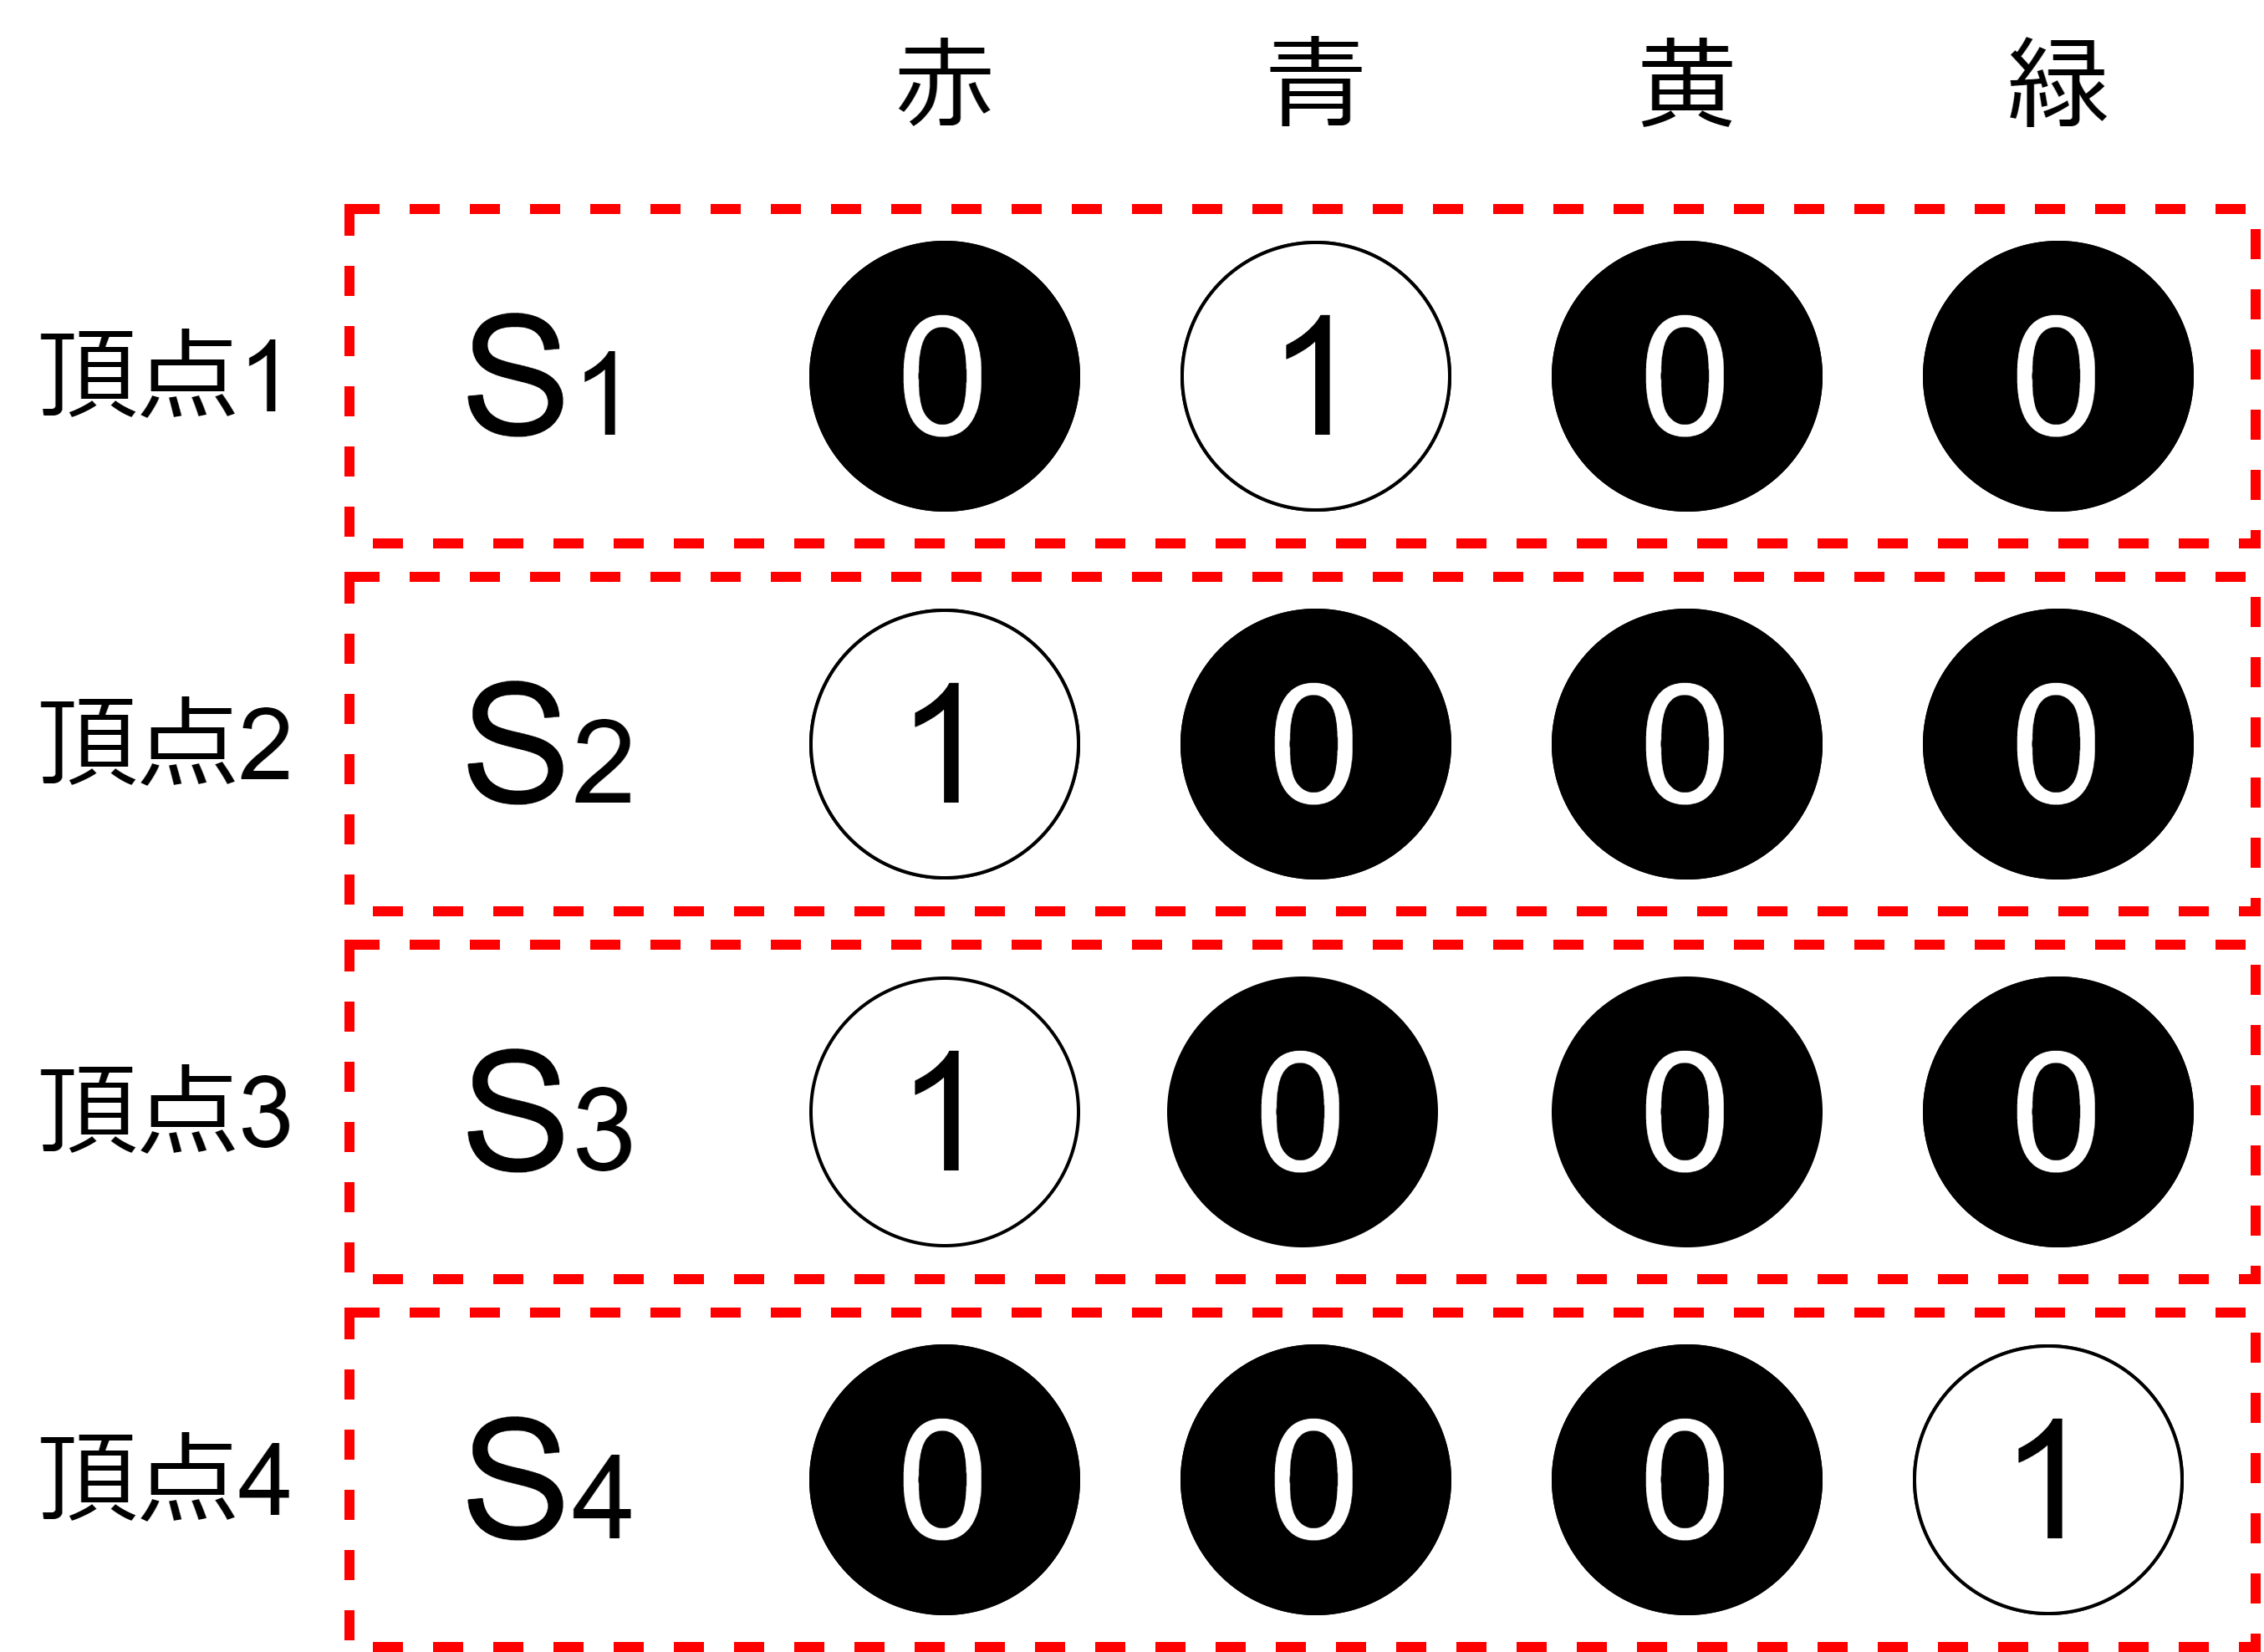
\includegraphics[width=0.9\linewidth]{data/GCP_example}
      \end{column}
      \begin{column}{0.45\linewidth}
        \centering
        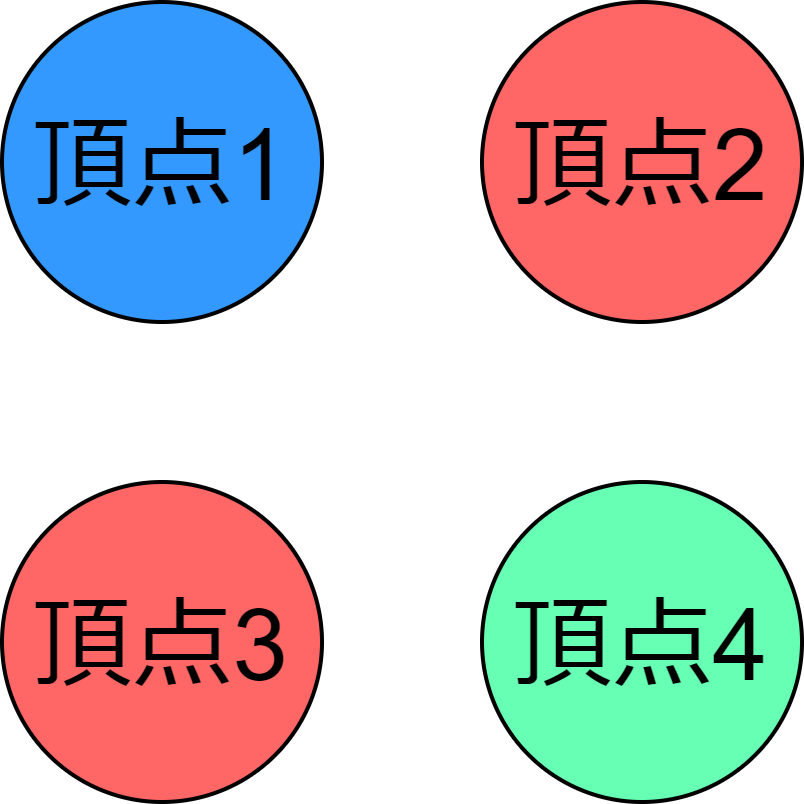
\includegraphics[width=0.5\linewidth]{data/GCP_example_graph}    
      \end{column}
    \end{columns}
  \end{figure}
\end{frame}

\begin{frame}
  \frametitle{状態遷移方法}
  \begin{columns}
    \begin{column}{0.6\linewidth}
  \begin{figure}[h]
    \centering
    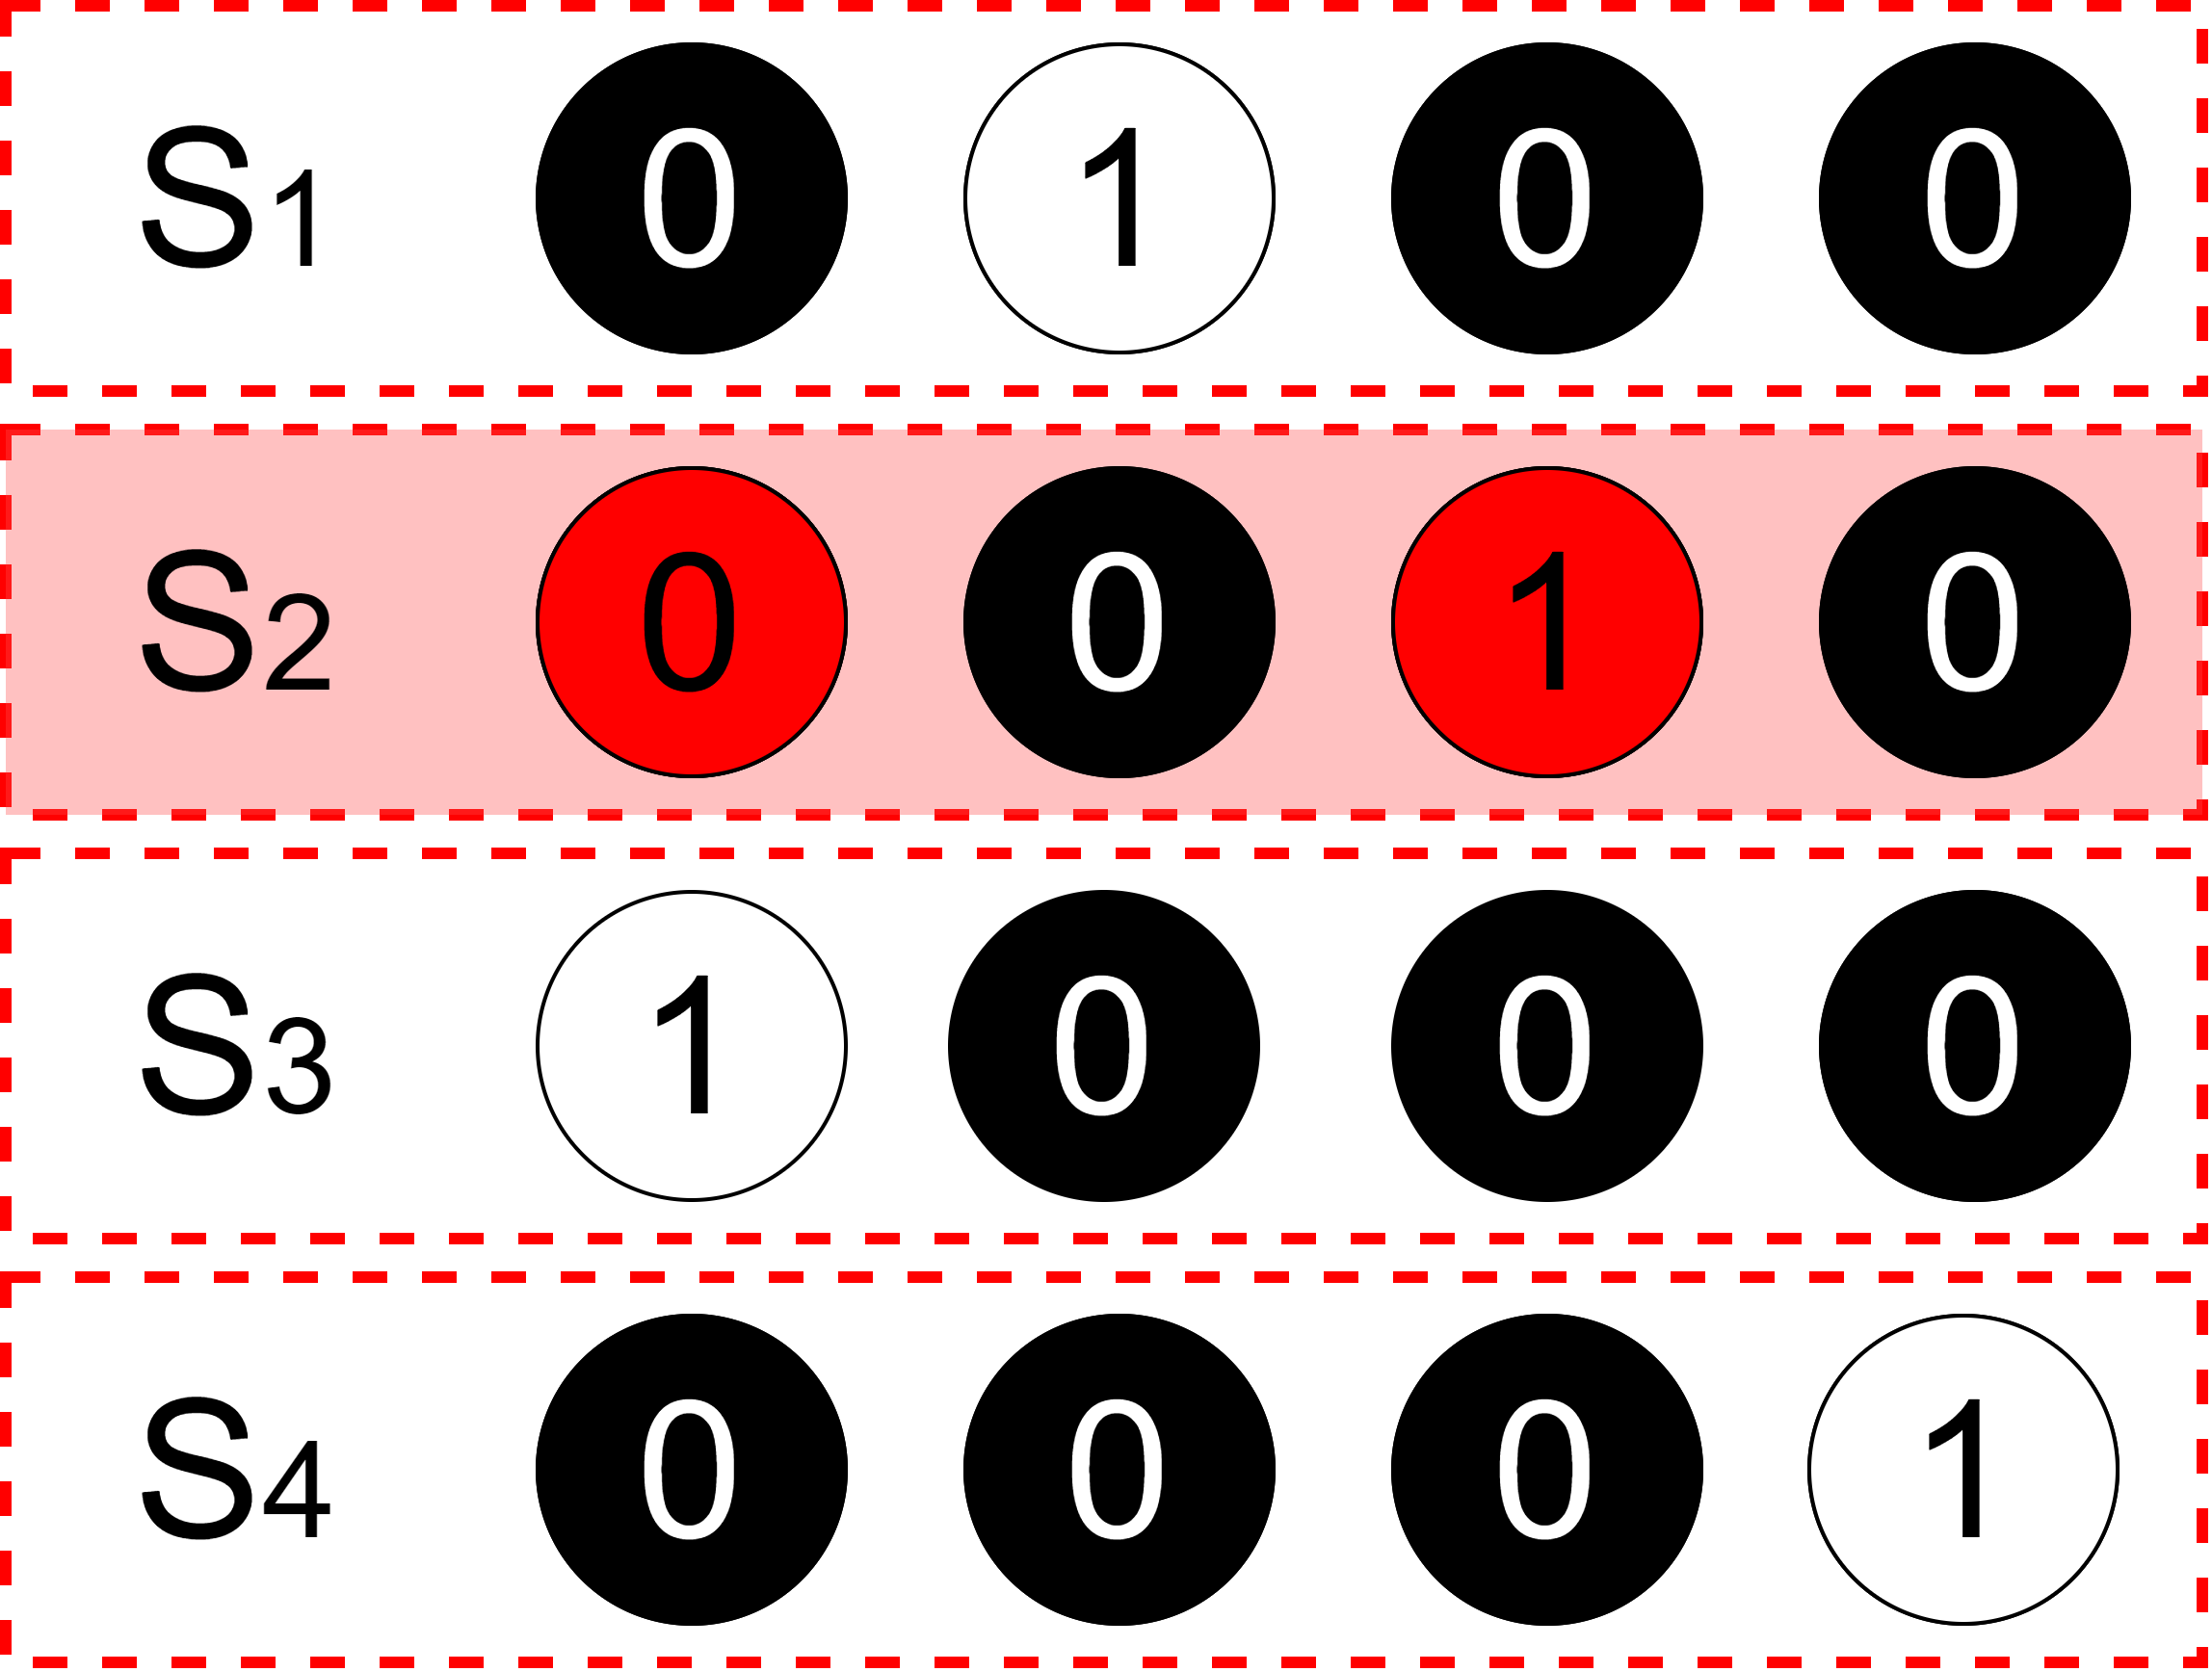
\includegraphics[width=0.8\linewidth]{data/kanzen1ji_bitflip}
  \end{figure}
    \end{column}
    \begin{column}{0.4\linewidth}
      \begin{enumerate}
        \item $S_i$を一つ選ぶ
        \item 0と1を交換する
        \item 状態遷移完了
      \end{enumerate}
    \end{column}
  \end{columns}
\end{frame}

\begin{frame}
  \frametitle{その次くらいに有名な例:巡回セールスマン}
  \begin{figure}[h]
    \begin{columns}
      \begin{column}{0.55\linewidth}        
        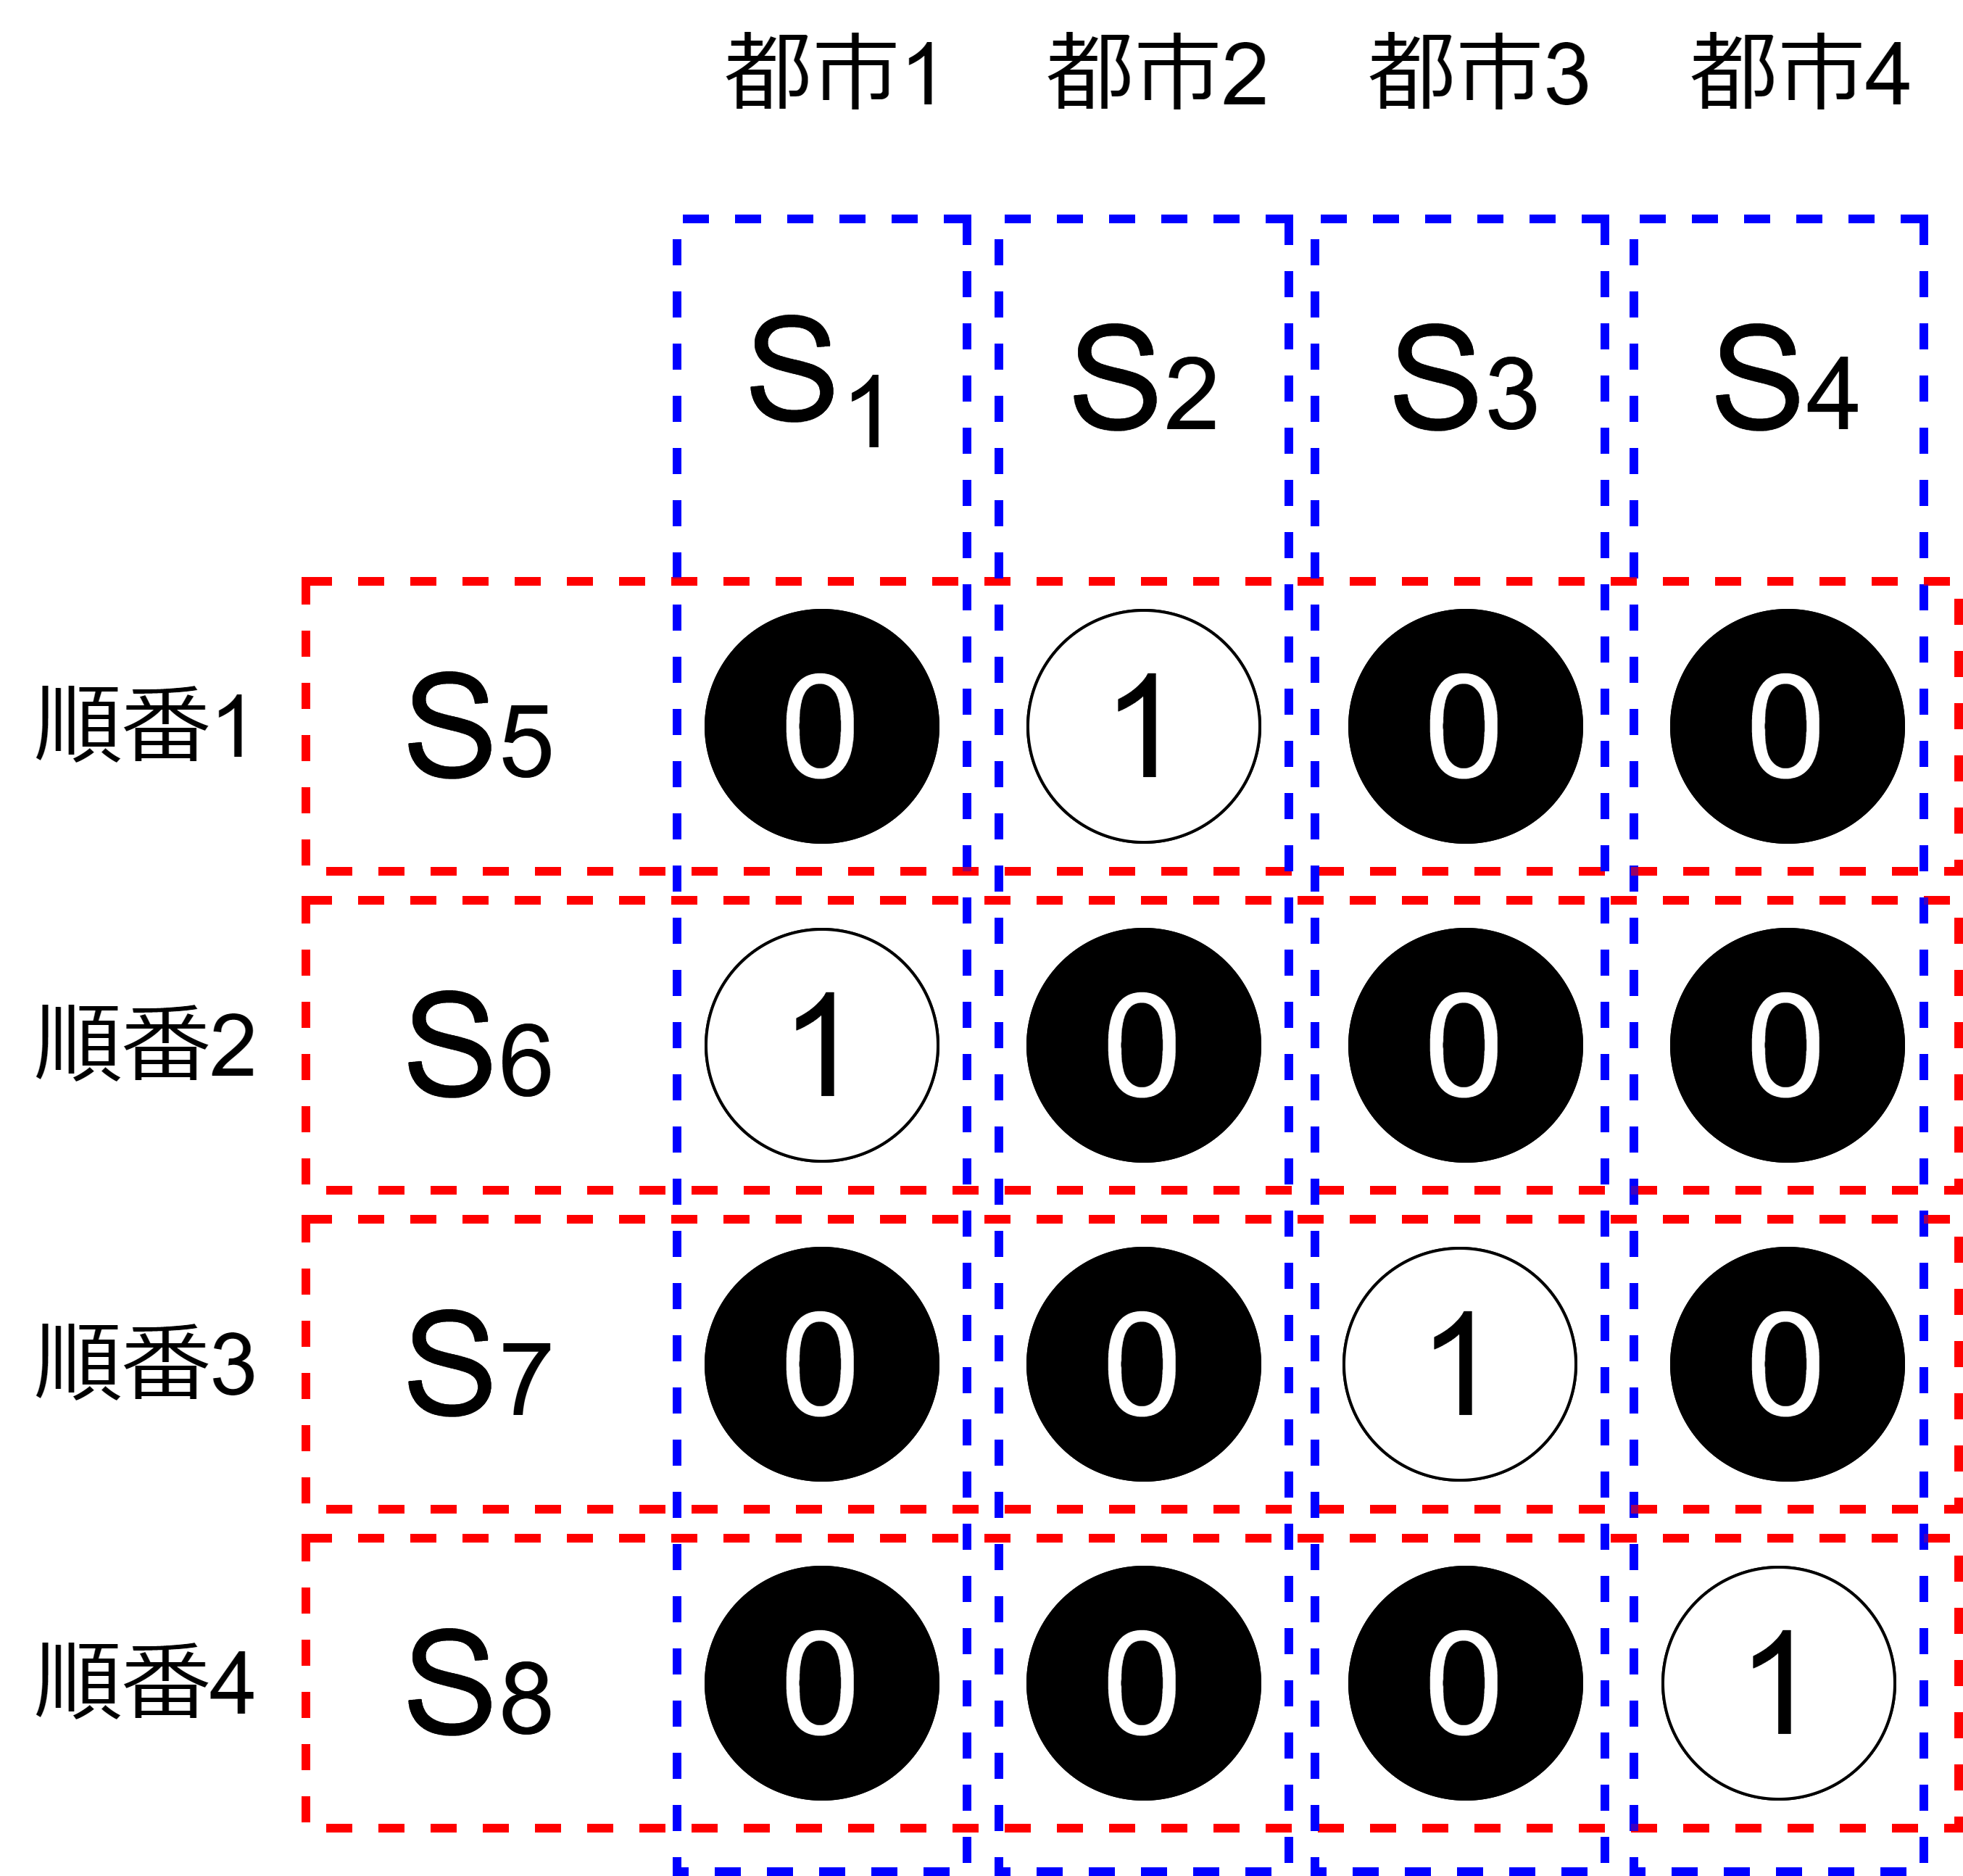
\includegraphics[width=0.9\linewidth]{data/TSP_example}
      \end{column}
      \begin{column}{0.45\linewidth}
        \centering
        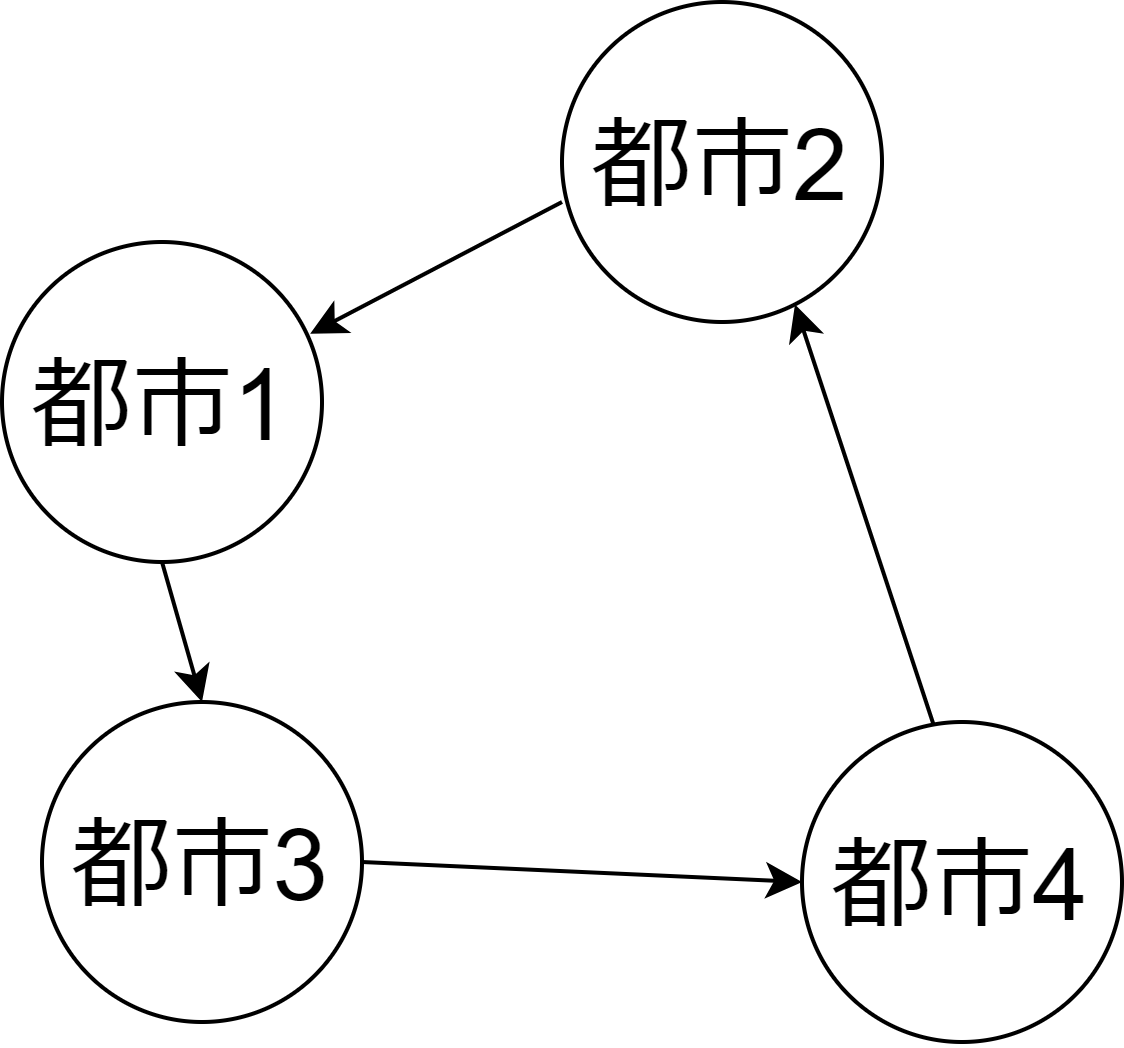
\includegraphics[width=0.8\linewidth]{data/TSP_example_graph}    
      \end{column}
    \end{columns}
  \end{figure}
\end{frame}

\begin{frame}
  \frametitle{状態遷移方法}
  \begin{columns}
    \begin{column}{0.6\linewidth}
  \begin{figure}[h]
    \centering
    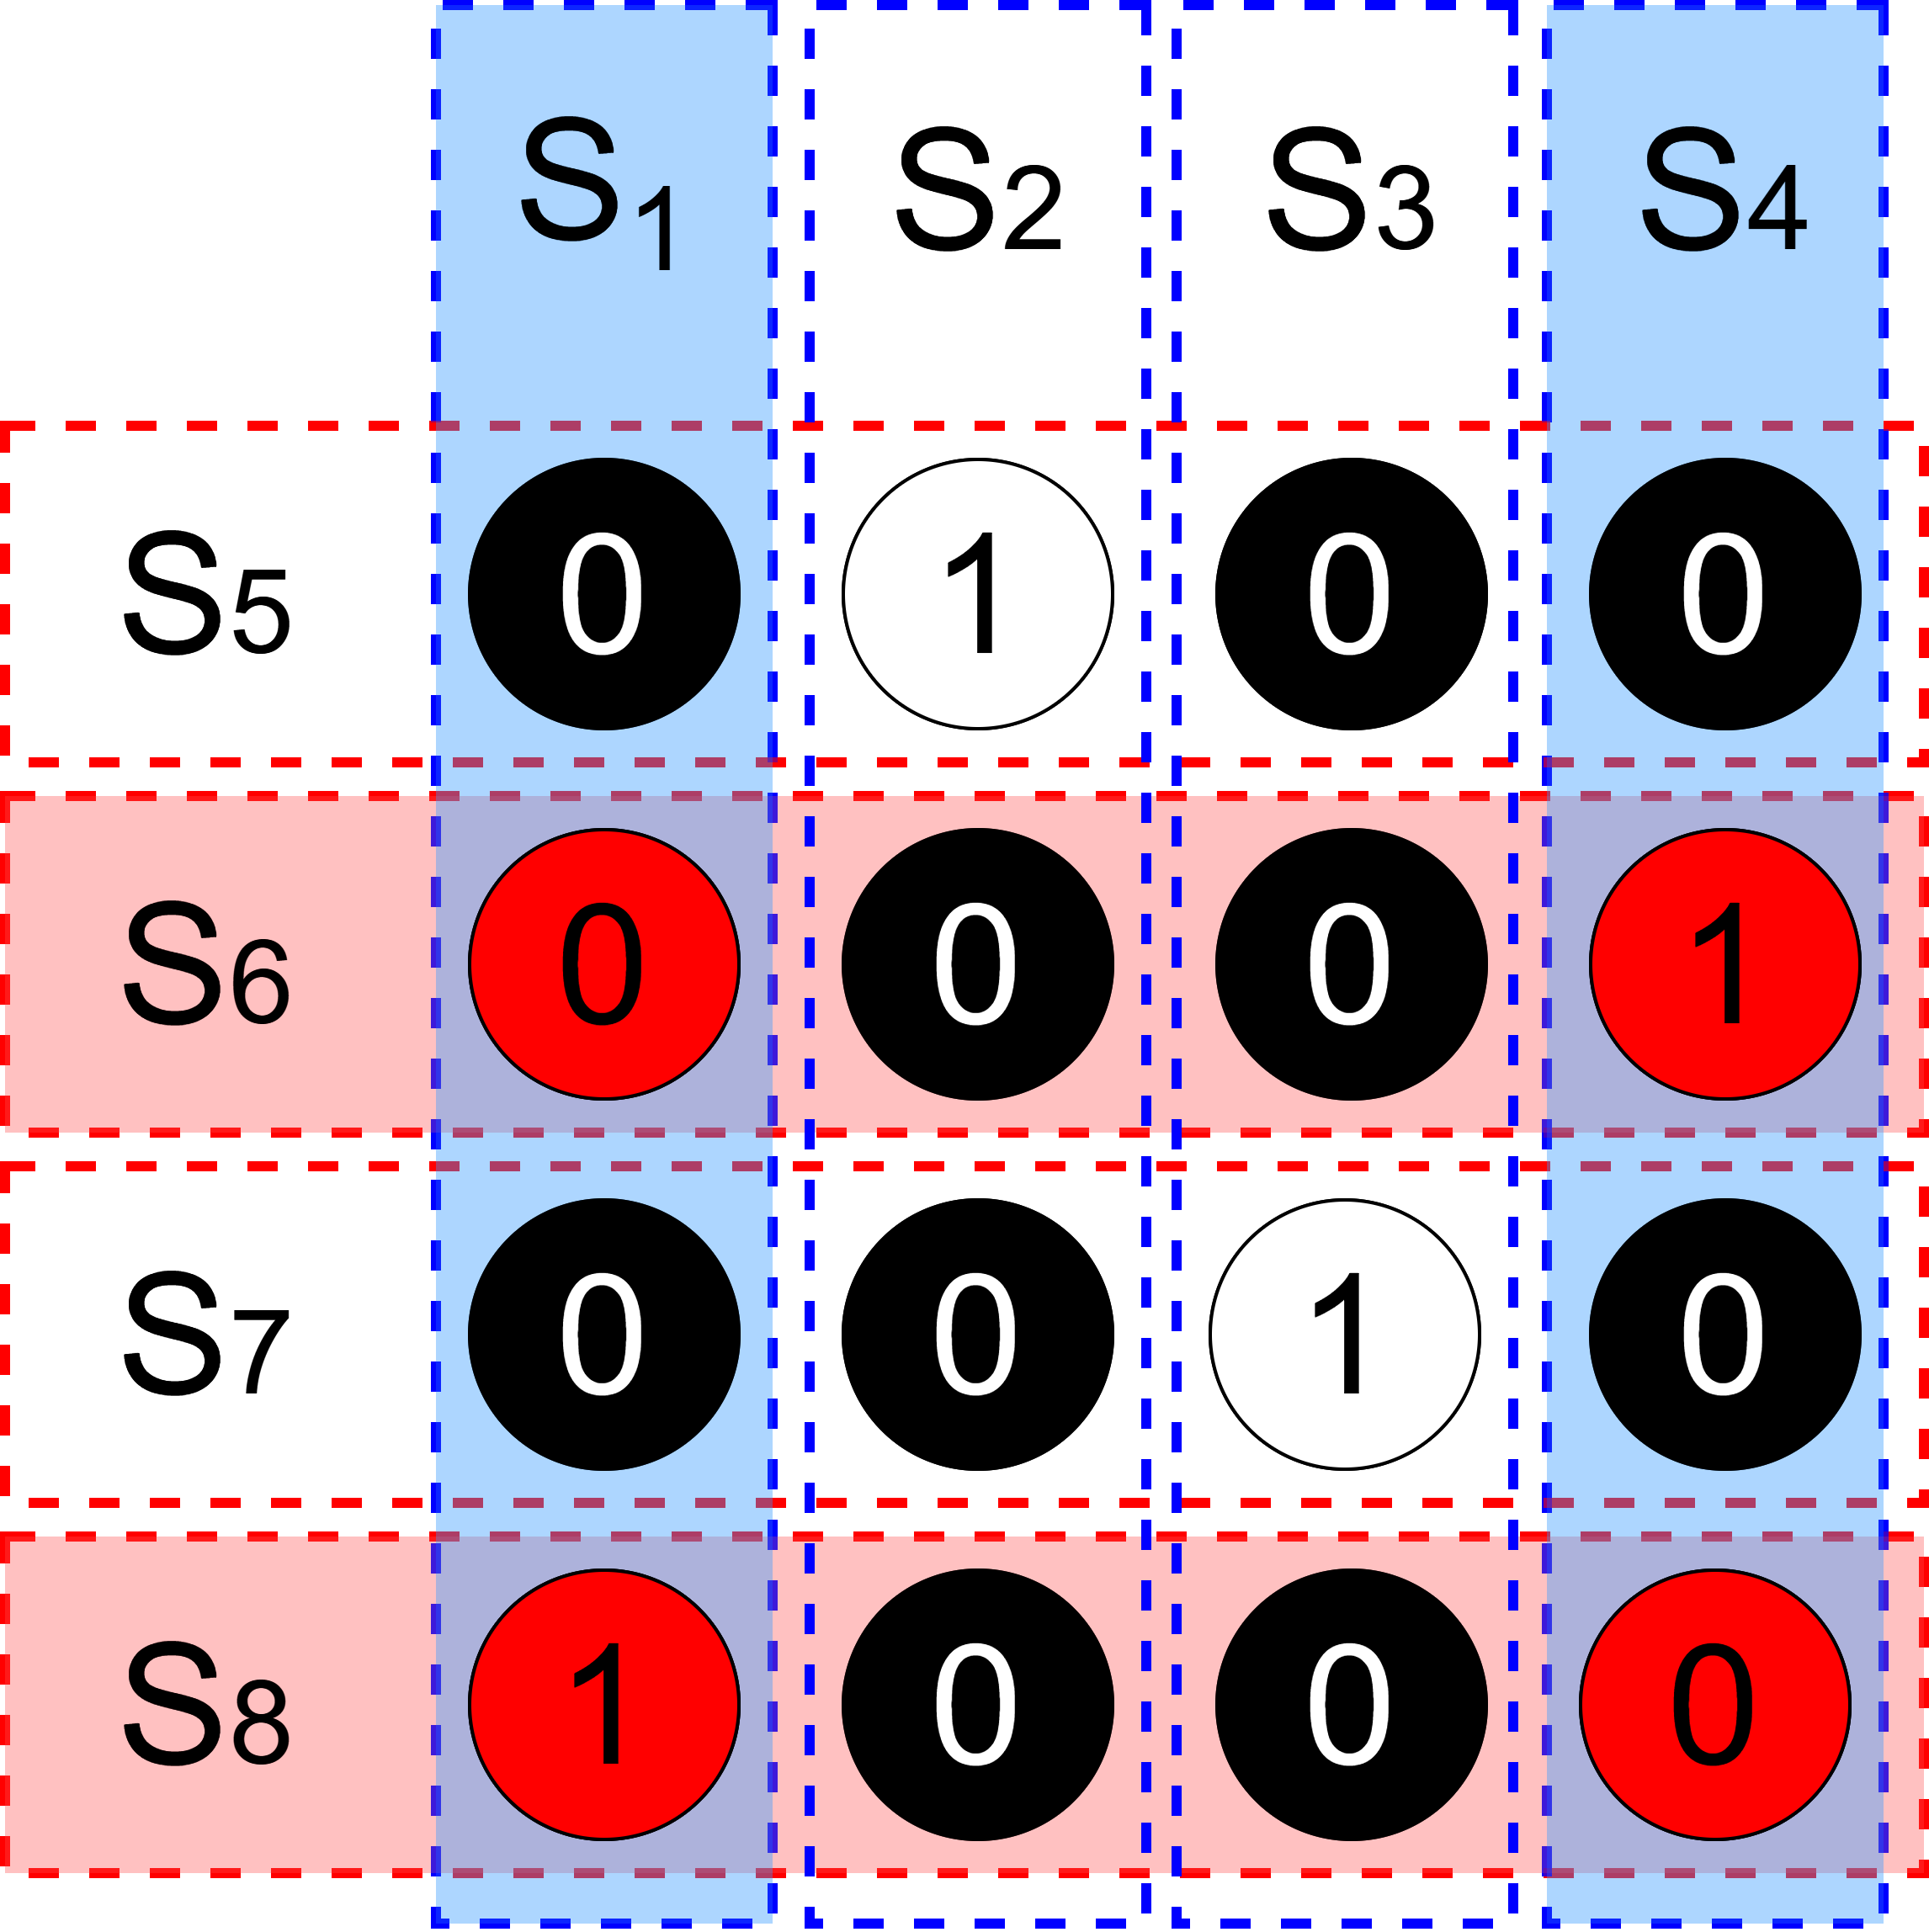
\includegraphics[width=0.8\linewidth]{data/kanzen2ji_bitflip}
  \end{figure}
    \end{column}
    \begin{column}{0.4\linewidth}
      \begin{enumerate}
        \item 2列$\left(S_i(1\leq i \leq 4)\right)$選ぶ
        \item 1を含む行を2行選ぶ
        \item 選んだ列・行の交点の4ビットをフリップ
        \item 状態遷移完了
      \end{enumerate}
    \end{column}
  \end{columns}
\end{frame}

% \section{比較}
% \begin{frame}
%   \frametitle{比較:n-彩色問題}
%   \begin{figure}
%     \begin{columns}
%       \begin{column}{0.47\linewidth}
%         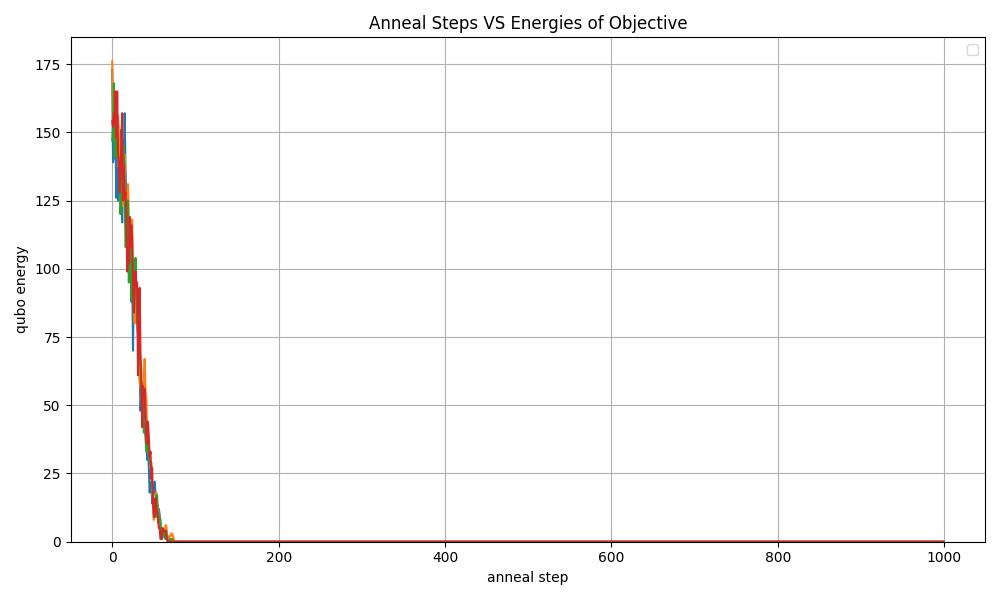
\includegraphics[width=1\linewidth]{data/GC_ene.png}
%         \caption{Swap basedのQAS}        
%       \end{column}
%       \begin{column}{0.47\linewidth}
%         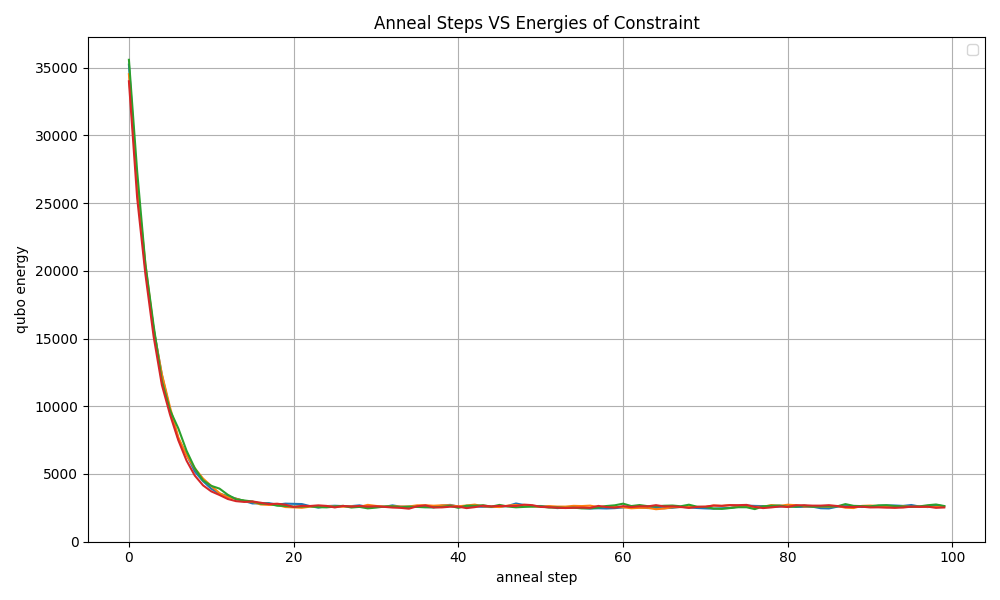
\includegraphics[width=1\linewidth]{data/GC_onehot_ene.png}
%         \caption{普通のQAS}
%       \end{column}
%     \end{columns}
%   \end{figure}
%   ※縦軸の目盛りが異なることに注意
% \end{frame}

% \begin{frame}
%   \frametitle{比較:巡回セールスマン}
%   \begin{figure}
%     \begin{columns}
%       \begin{column}{0.47\linewidth}
%         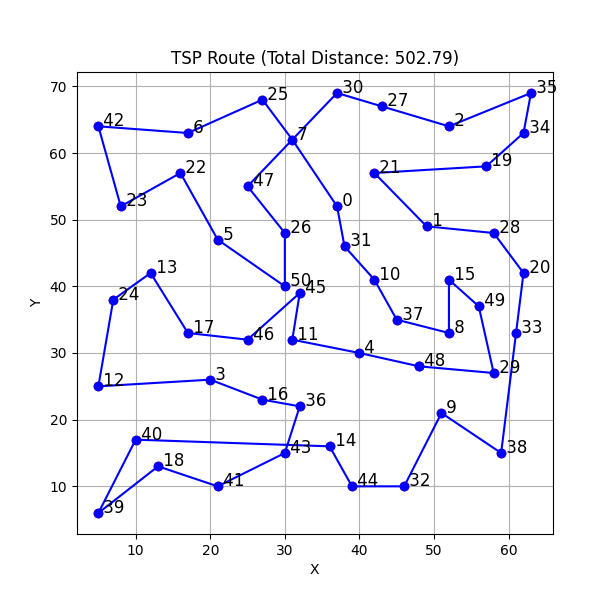
\includegraphics[width=1\linewidth]{data/TSP_graph.png}
%         \caption{Swap basedのQAS (energy = 502.79)}        
%       \end{column}
%       \begin{column}{0.47\linewidth}
%         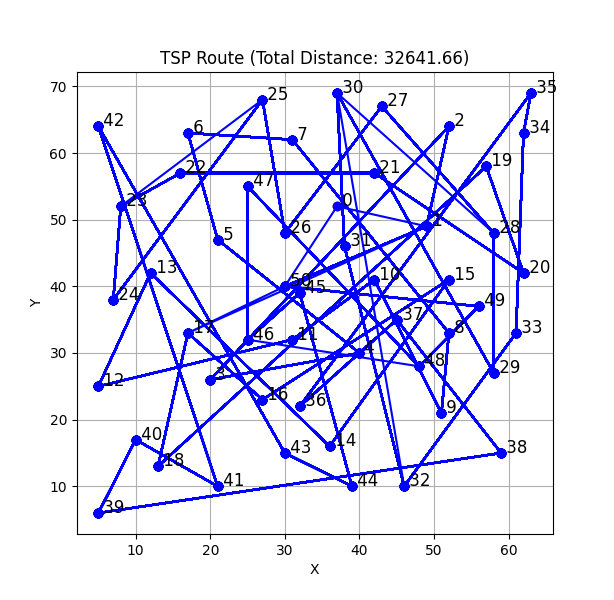
\includegraphics[width=1\linewidth]{data/TSP_broken.png}
%         \caption{普通のQAS (energy = 32641.66)}
%       \end{column}
%     \end{columns}
%   \end{figure}
% \end{frame}

% \section{手法(再)}
\begin{frame}
  \frametitle{グラフで表現する}
  \begin{figure}
    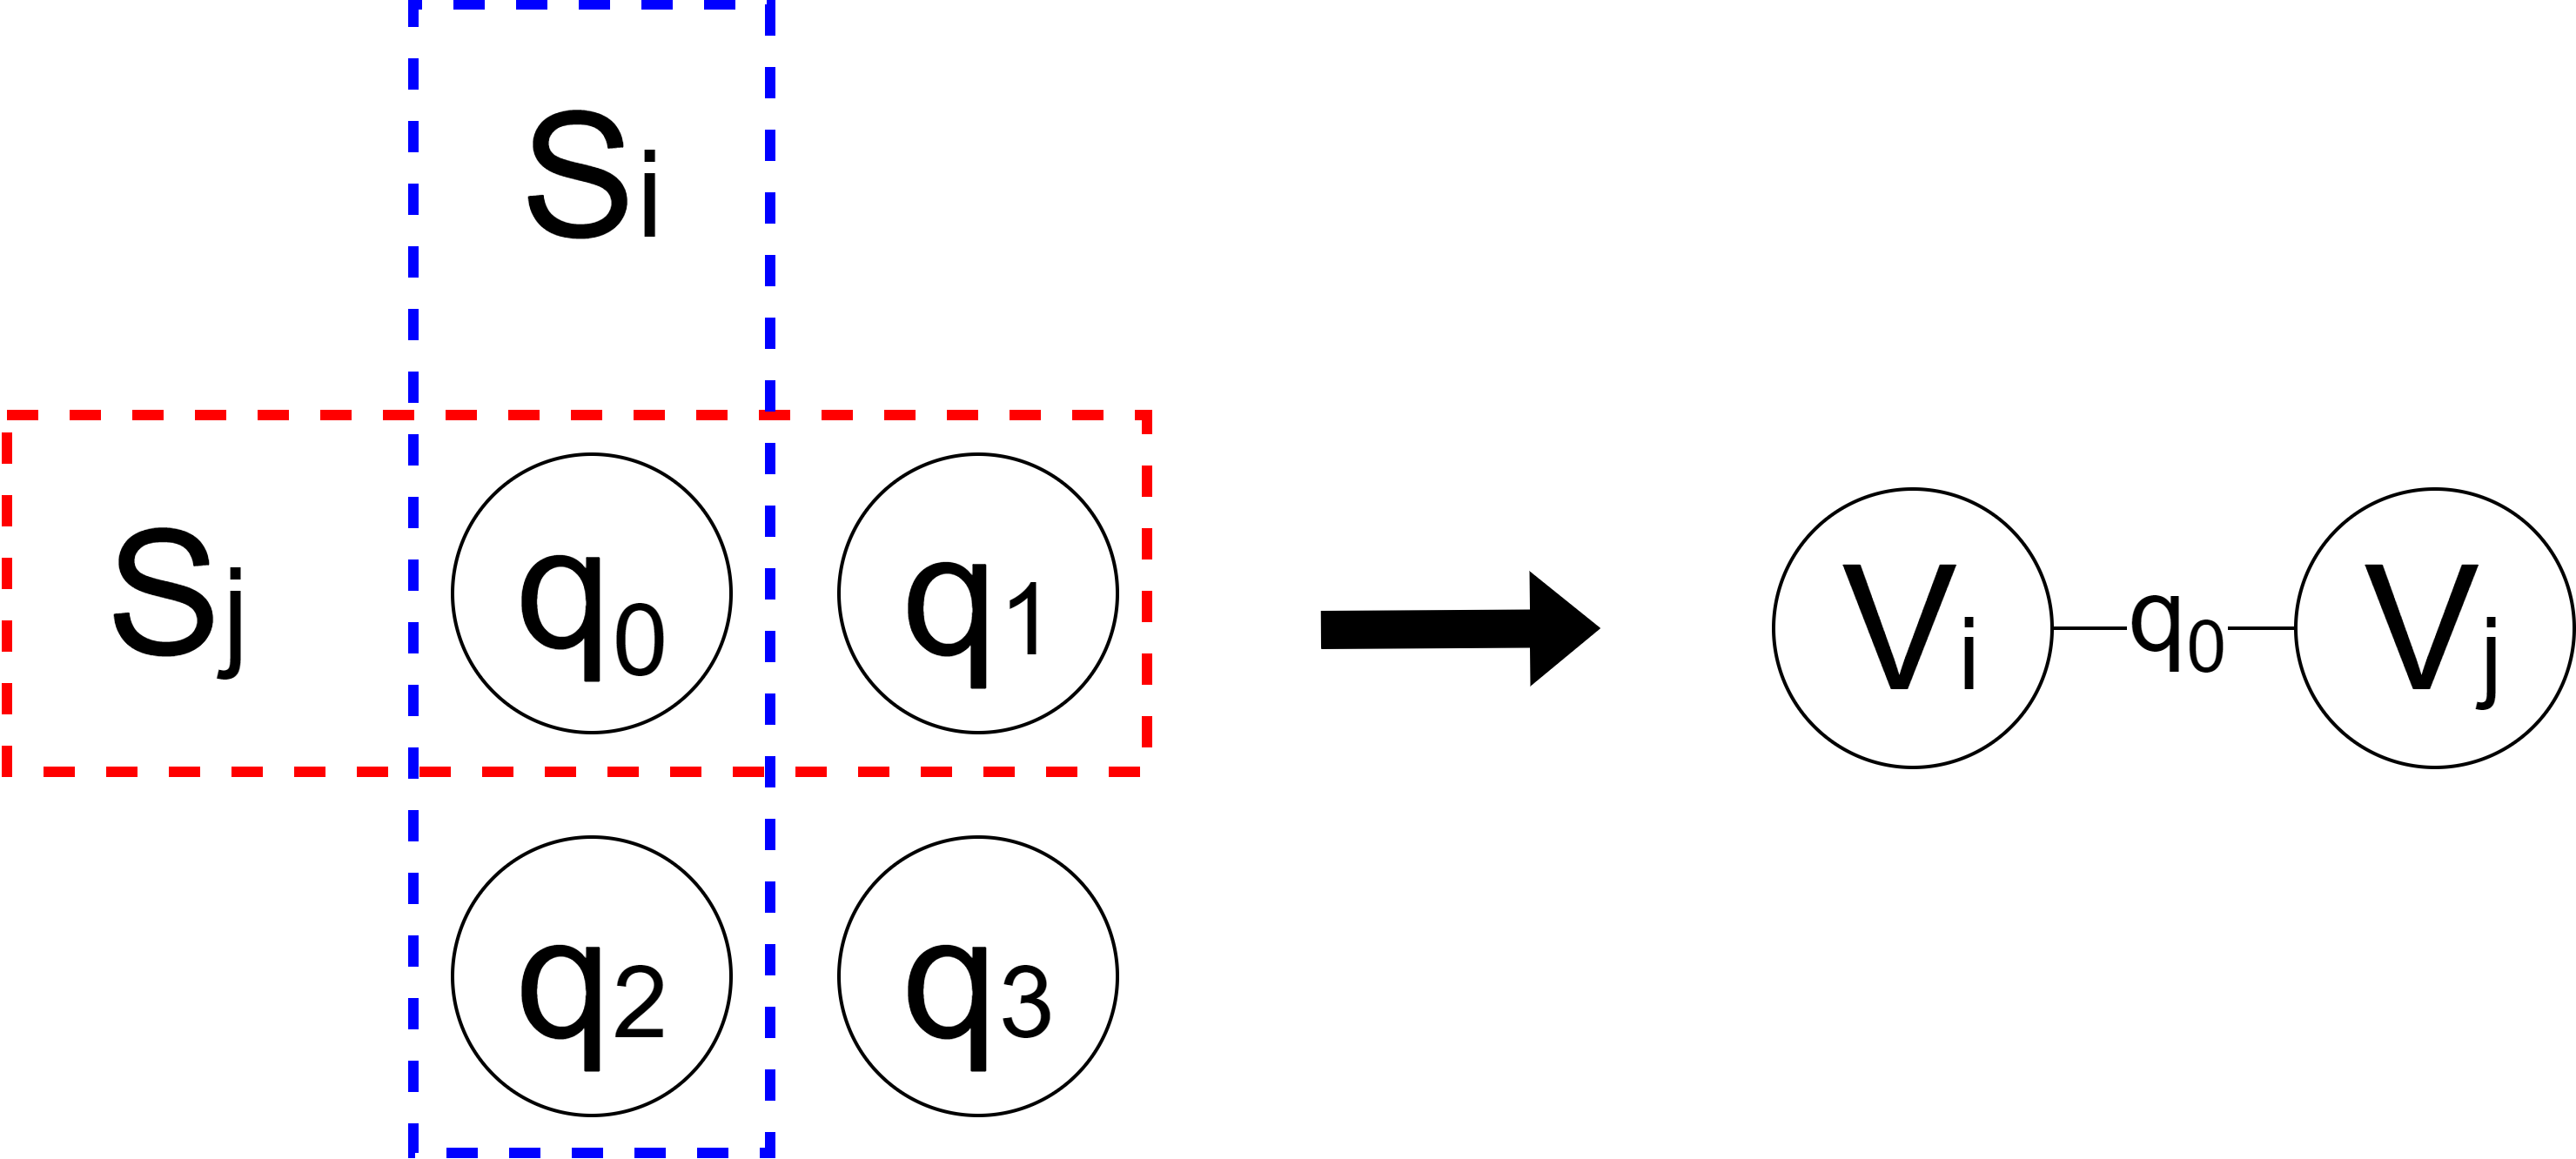
\includegraphics[width=0.8\linewidth]{data/bit_to_graph.png}
  \end{figure}
  \centering
  $S_i\cap S_j = q_k \rightarrow V_i \text{と} V_j \text{間に重み}q_k\text{のエッジが存在}$
\end{frame}

\begin{frame}
  \frametitle{n-彩色問題再論}
  \begin{figure}
      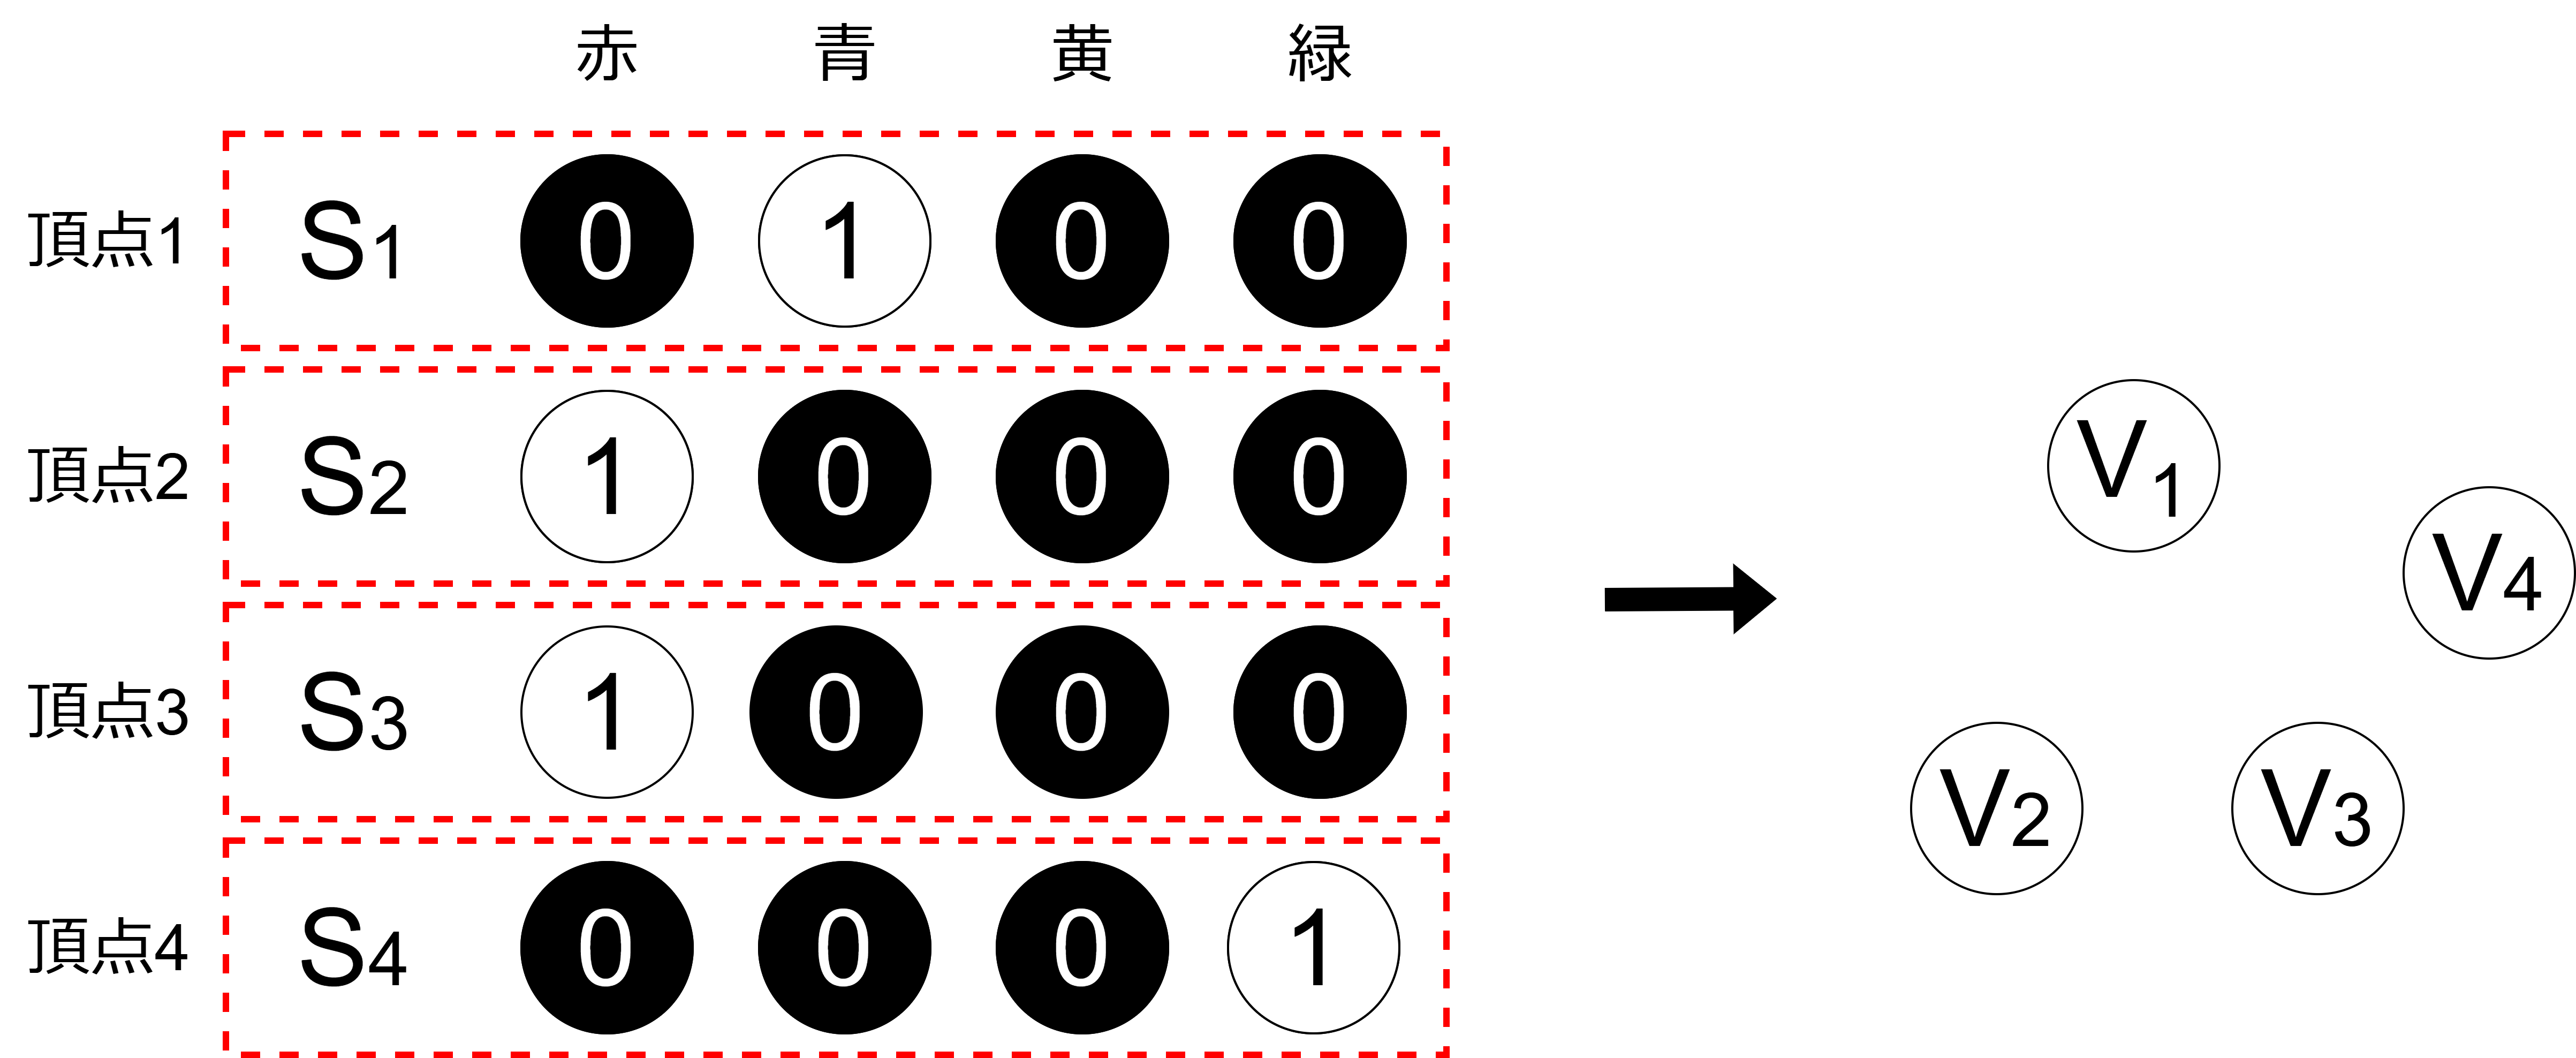
\includegraphics[width=0.85\linewidth]{data/kanzen1ji_to_graph}
  \end{figure}

\end{frame}

\begin{frame}
  \frametitle{巡回セールスマン問題再論}
  \begin{figure}
      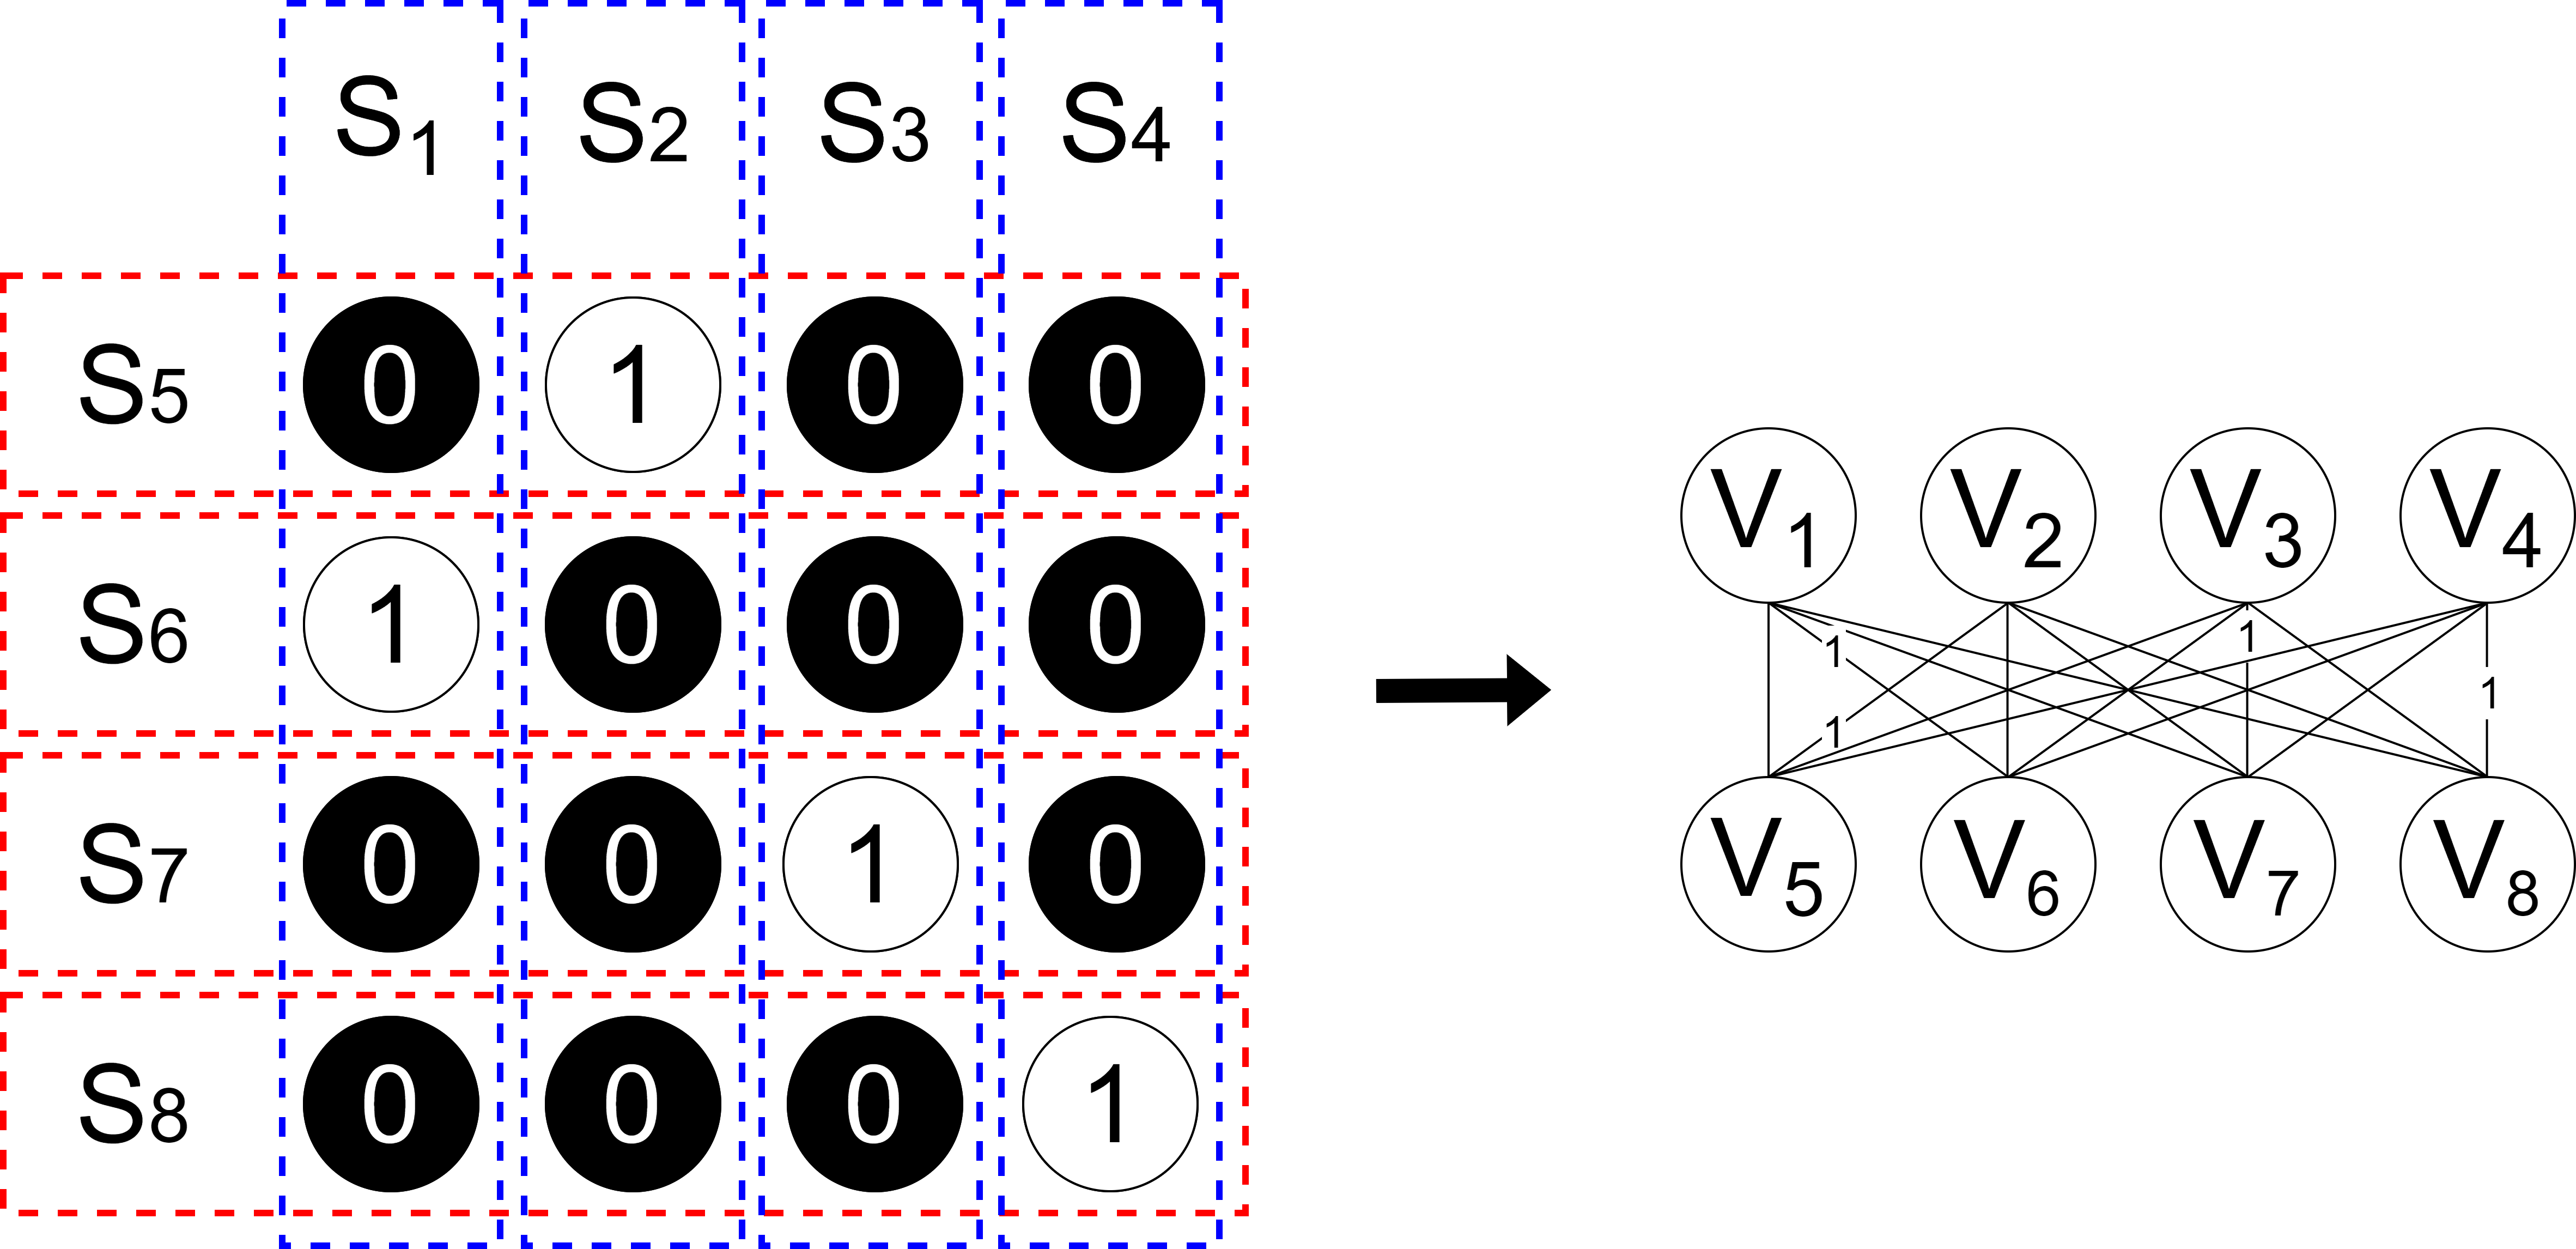
\includegraphics[width=0.85\linewidth]{data/kanzen2ji_to_graph}
  \end{figure}
  \rightline{\small{(重みは1のみ明記、0は省略)}}
  \centering
  多くの問題が完全二部グラフに相当する
\end{frame}

\begin{frame}
  \frametitle{こんな問題は見たことないが}
  \begin{figure}
      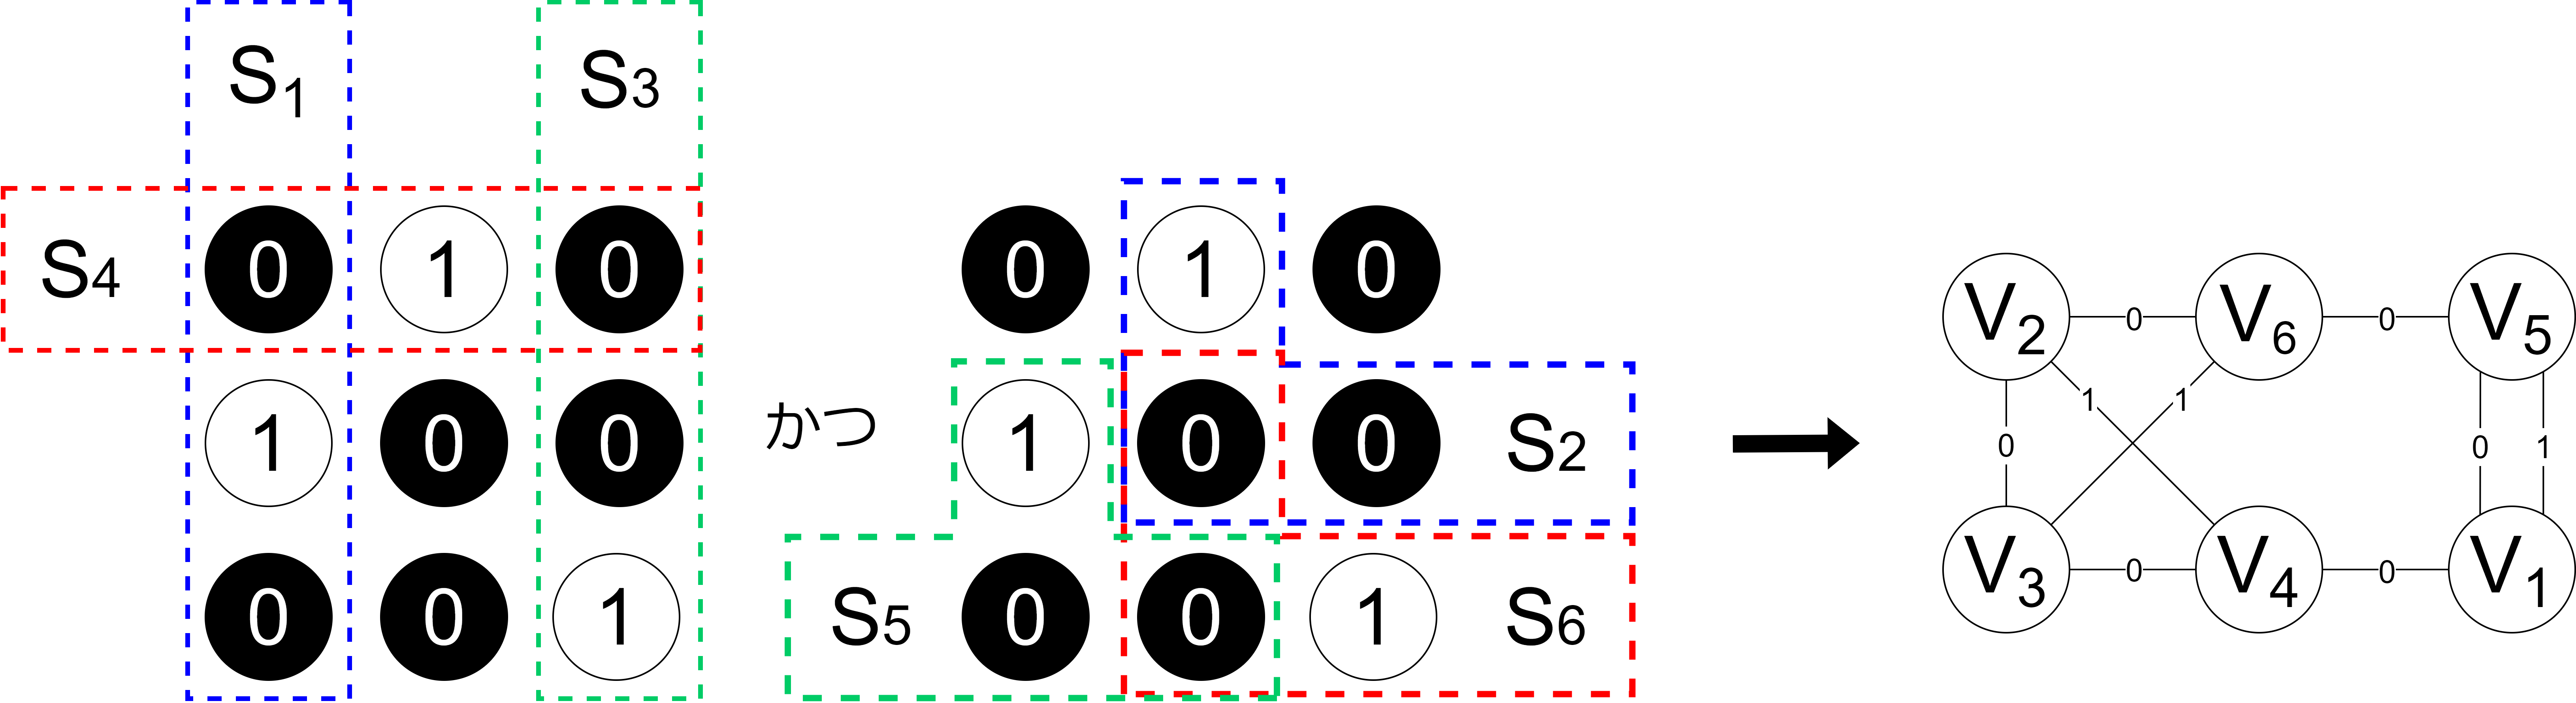
\includegraphics[width=1\linewidth]{data/2ji_to_graph}
  \end{figure}
\end{frame}

\begin{frame}
  \frametitle{グラフで表現したことによる嬉しさ}
  \begin{figure}
    \begin{columns}
      \begin{column}{0.47\linewidth}
        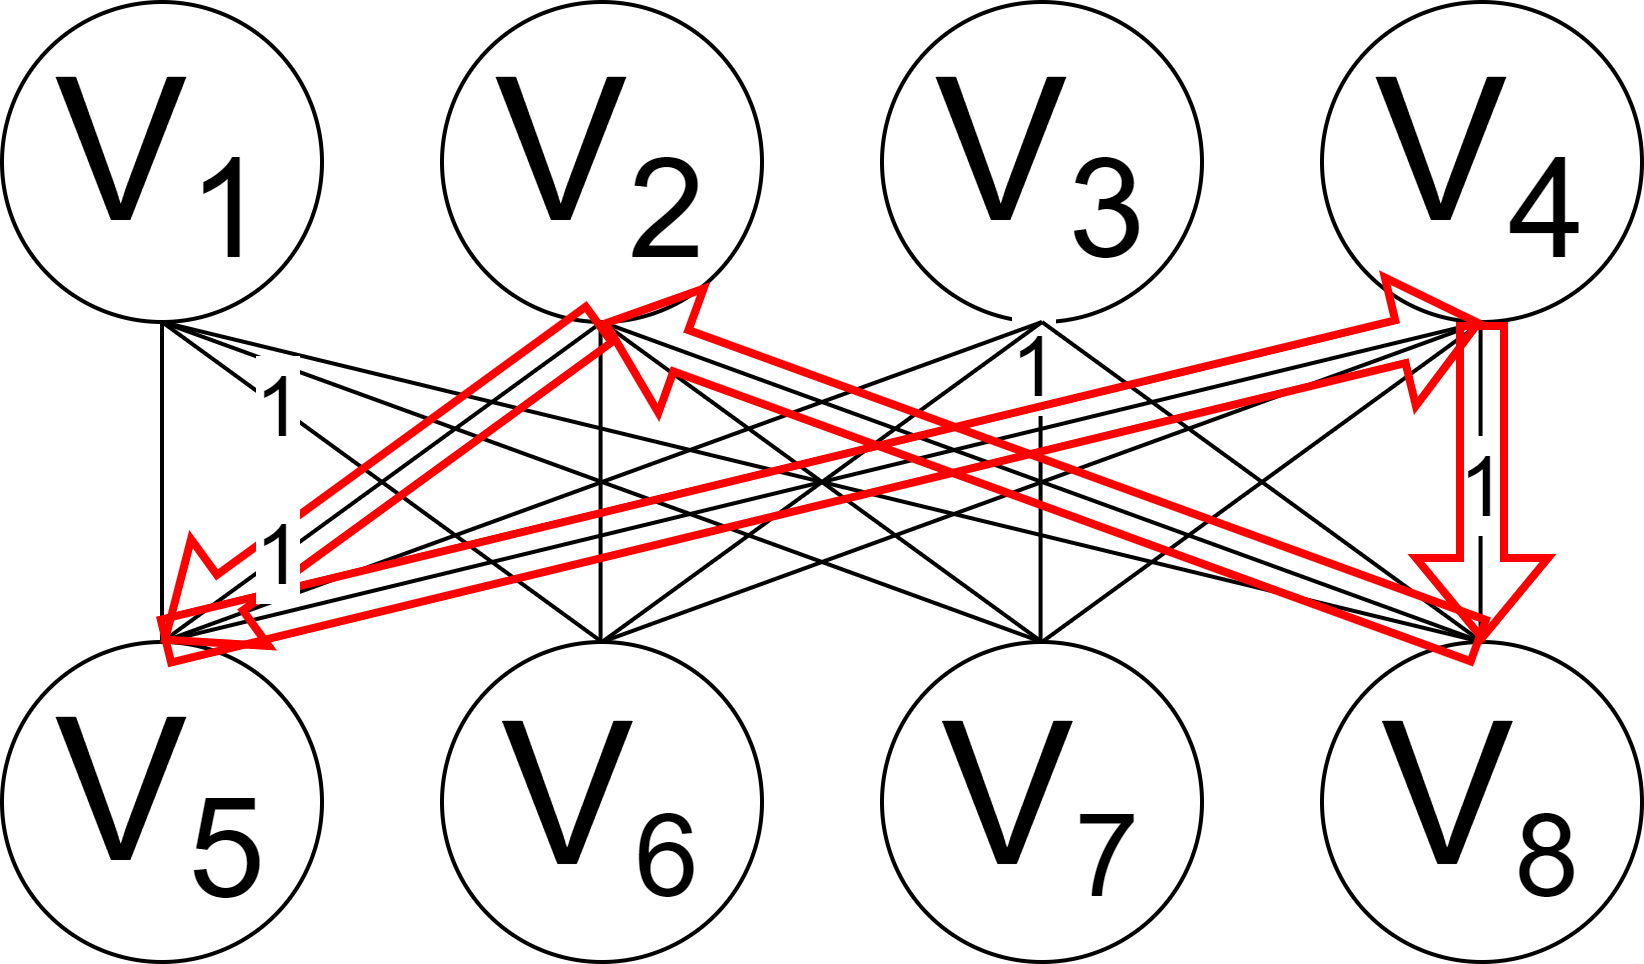
\includegraphics[width=1\linewidth]{data/kanzen2ji_path.png}     
      \end{column}
      \begin{column}{0.47\linewidth}
        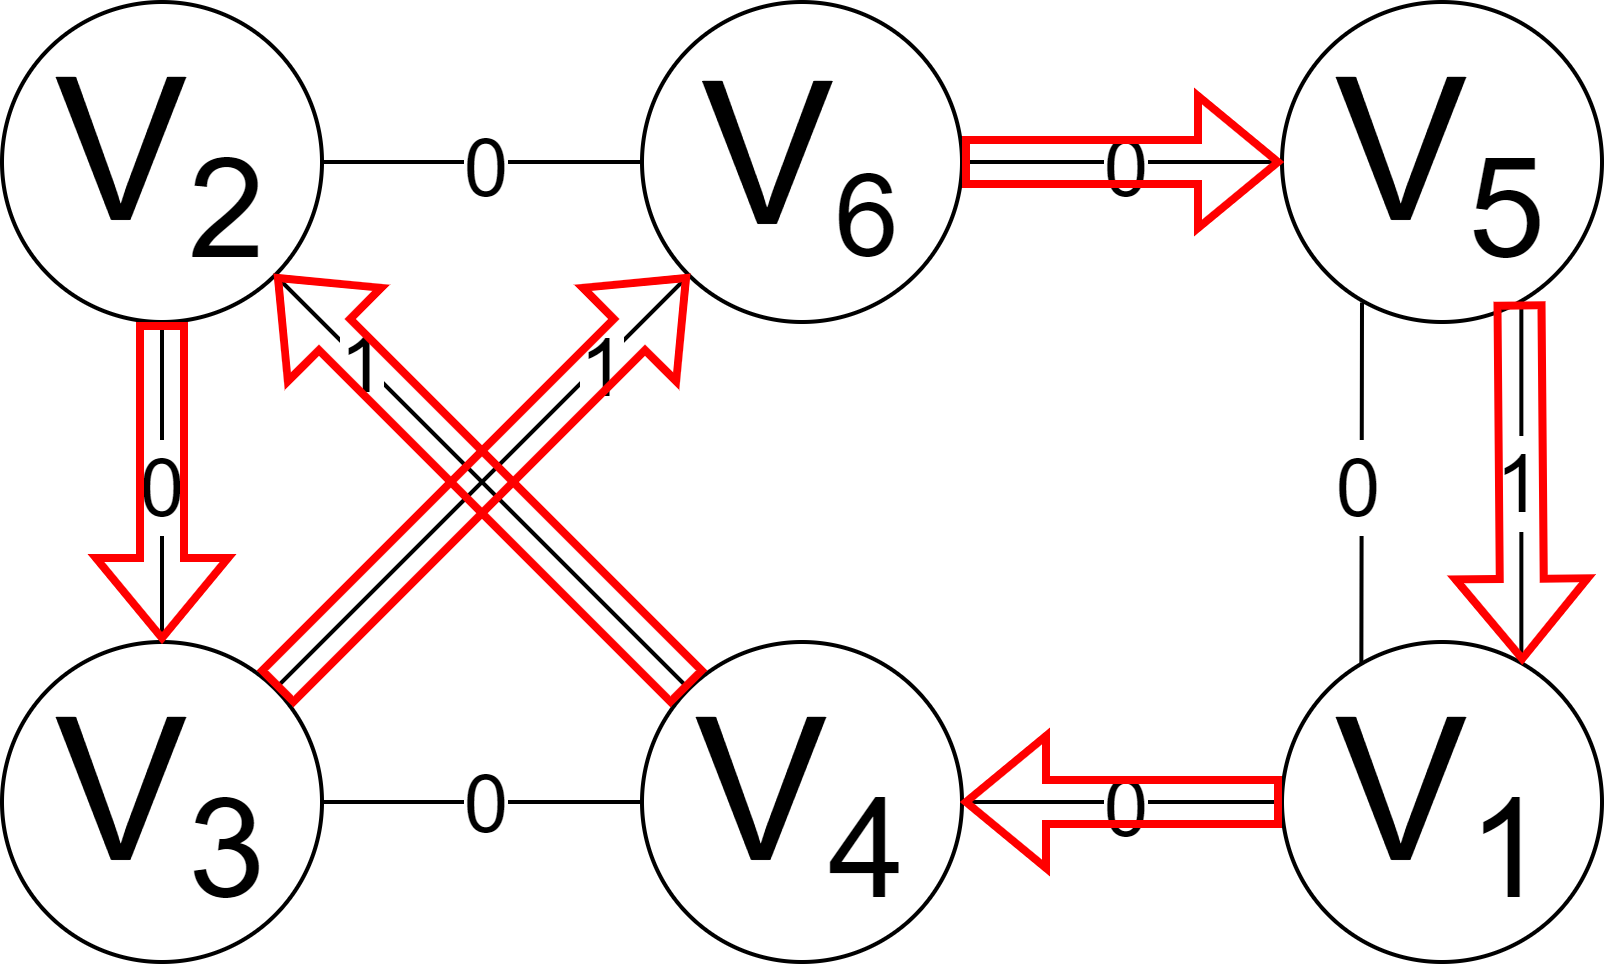
\includegraphics[width=1\linewidth]{data/2ji_path.png}
      \end{column}
    \end{columns}
  \end{figure}
  \centering
  問題によらず、ビットフリップ方法を統一的に説明できる
\end{frame}

\begin{frame}
  \frametitle{ビットフリップ方法}
    \begin{columns}
      \begin{column}{0.47\linewidth}
        \begin{figure}
          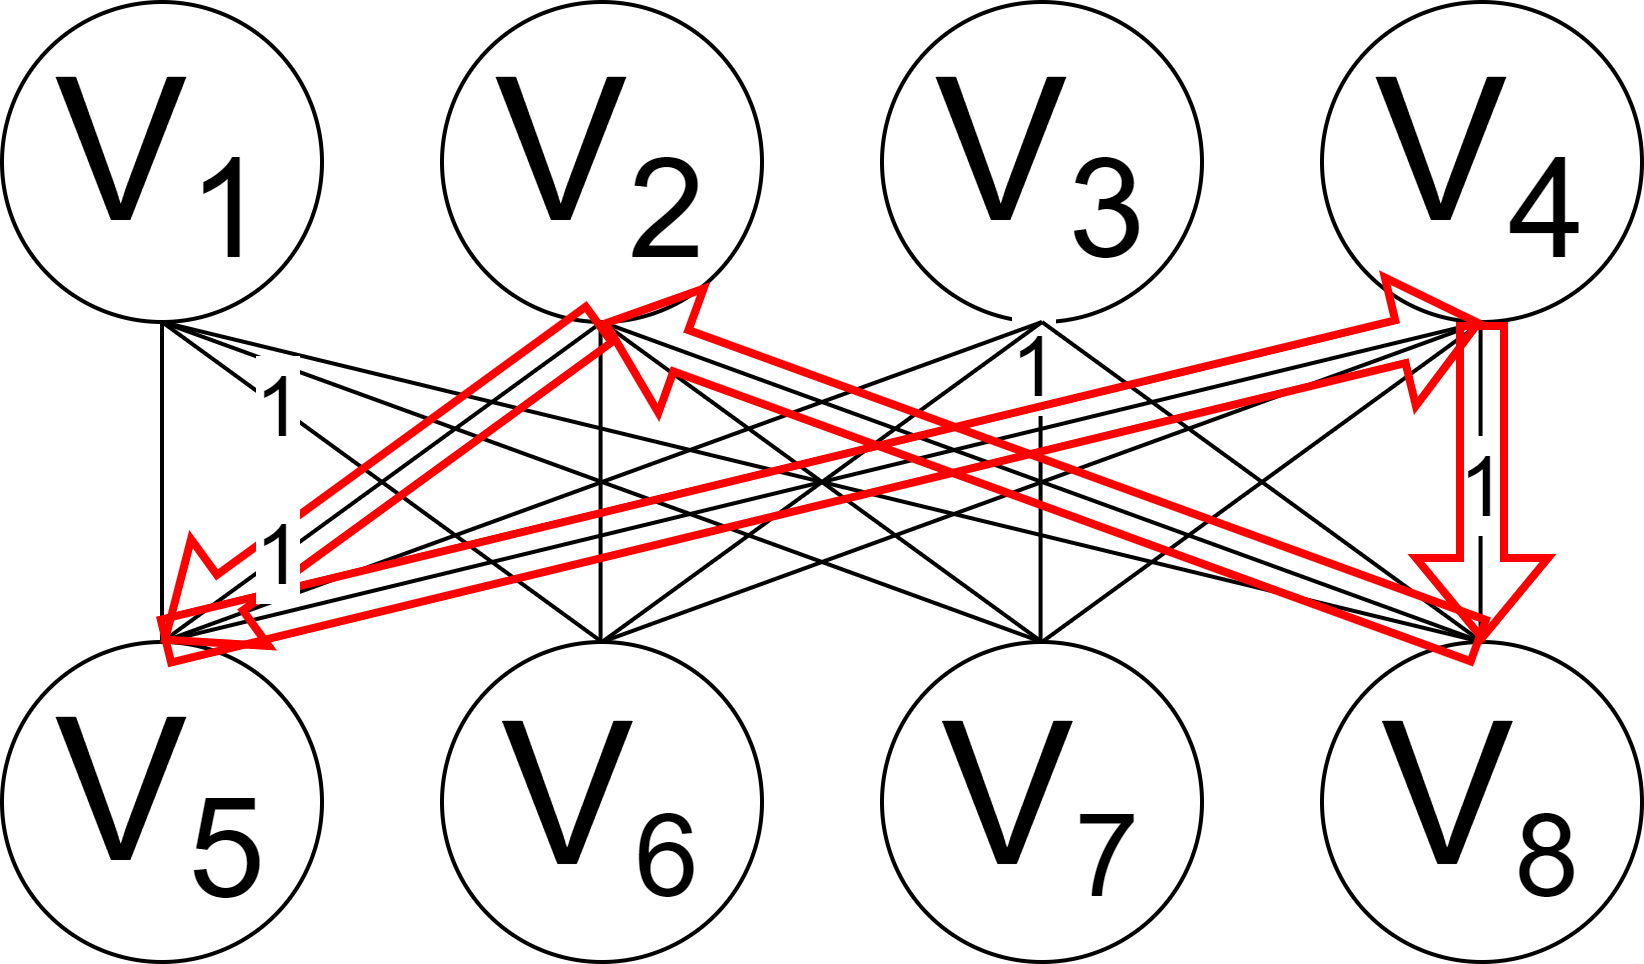
\includegraphics[width=1\linewidth]{data/kanzen2ji_path.png}       
        \end{figure}
      \end{column}
      \begin{column}{0.47\linewidth}
          \begin{enumerate}
            \item 条件を満たす閉路を探索する
            \begin{itemize}
              \item 偶閉路
              \item 重み0,1のエッジを交互に通る
            \end{itemize}
            \item 閉路上のエッジの重みをすべてフリップする
            \item ビットの値をエッジの重みに対応するように更新
          \end{enumerate}
      \end{column}
    \end{columns}
\end{frame}

\section{展望}
\begin{frame}
  \frametitle{これからしたいこと}
  \begin{itemize}
    \item 一般化された制約条件下での条件を満たす閉路を探索するフェーズの考察
    \item より高次の制約条件への適用のための考察
  \end{itemize}
\end{frame}

\begin{frame}[allowframebreaks]{参考文献}
  \nocite{nishimori_ohzeki_quantum_annealing_basics}
  \nocite{hen2016driver}
  \nocite{hen2016quantum}
  \nocite{Morita_2008}
  \nocite{Openjij}
  \nocite{村田幸弘2007ペナルティ法による目的関数生成における重み付け自動化}
  \bibliographystyle{unsrt}
  \bibliography{bibliography.bib}

\end{frame}



